\documentclass[aps,pra,reprint,superscriptaddress,longbibliography,nofootinbib,floatfix,10pt]{revtex4-2}
\usepackage[T1]{fontenc}
\usepackage[utf8]{inputenc}
\usepackage{lmodern,amsmath,amssymb,amsthm,mathtools,bm,graphicx,booktabs,longtable,tikz,placeins,needspace,microtype}
\usepackage[dvipsnames]{xcolor}
\usetikzlibrary{calc,arrows.meta,positioning,fit,backgrounds}
\usepackage[colorlinks=true,linkcolor=blue,citecolor=blue,urlcolor=blue,breaklinks=true]{hyperref}
\usepackage{orcidlink}

\newtheorem{theorem}{Theorem}
\newtheorem{lemma}[theorem]{Lemma}
\newtheorem{proposition}[theorem]{Proposition}
\newtheorem{corollary}[theorem]{Corollary}
\theoremstyle{definition}\newtheorem{definition}[theorem]{Definition}
\theoremstyle{remark}\newtheorem{remark}[theorem]{Remark}

\newcommand{\C}{\mathbb C}\newcommand{\R}{\mathbb R}\newcommand{\Q}{\mathbb Q}
\newcommand{\F}{\mathbb F}\newcommand{\Z}{\mathbb Z}\newcommand{\PP}{\mathbb P}
\newcommand{\Sc}{\mathcal S}\newcommand{\Cc}{\mathcal C}\newcommand{\Wc}{\mathcal W}
\newcommand{\YO}{\mathrm{YO}}\newcommand{\ip}[2]{\langle #1,#2\rangle}
\newcommand{\Htwenty}{\mathsf H_{20}}
\DeclareMathOperator{\spanop}{span}\DeclareMathOperator{\rank}{rank}
\DeclareMathOperator{\diag}{diag}\DeclareMathOperator{\Tr}{Tr}\DeclareMathOperator{\tr}{tr}
\DeclareMathOperator{\supp}{supp}\DeclareMathOperator{\conv}{conv}

% --- Inline TikZ palette and macros ---
\definecolor{YOtriad}{HTML}{246A9A}
\definecolor{YObasis}{HTML}{8A939B}
\definecolor{YOspoke}{HTML}{237D70}
\definecolor{YOouterA}{HTML}{85458B}
\definecolor{YOouterB}{HTML}{B47620}
\definecolor{YOdiagonal}{HTML}{B44850}
\colorlet{YOctx1}{YOtriad}
\colorlet{YOctx2}{YOtriad}
\colorlet{YOctx3}{YOtriad}
\colorlet{YOctx4}{YObasis}
\colorlet{YOctx5}{YOspoke}
\colorlet{YOctx6}{YOspoke}
\colorlet{YOctx7}{YOspoke}
\colorlet{YOctx8}{YOouterA}
\colorlet{YOctx11}{YOouterA}
\colorlet{YOctx16}{YOouterA}
\colorlet{YOctx9}{YOouterB}
\colorlet{YOctx13}{YOouterB}
\colorlet{YOctx14}{YOouterB}
\colorlet{YOctx10}{YOdiagonal}
\colorlet{YOctx12}{YOdiagonal}
\colorlet{YOctx15}{YOdiagonal}

\definecolor{ctx1}{RGB}{230,25,75}
\definecolor{ctx2}{RGB}{60,180,75}
\definecolor{ctx3}{RGB}{0,130,200}
\definecolor{ctx4}{RGB}{245,130,48}
\definecolor{ctx5}{RGB}{145,30,180}
\definecolor{ctx6}{RGB}{70,240,240}
\definecolor{ctx7}{RGB}{240,50,230}
\definecolor{ctx8}{RGB}{210,245,60}
\definecolor{ctx9}{RGB}{250,190,190}
\definecolor{ctx10}{RGB}{0,128,128}
\definecolor{ctx11}{RGB}{128,128,0}
\definecolor{ctx12}{RGB}{170,110,40}

\definecolor{colZero}{HTML}{D62728}
\definecolor{colOne}{HTML}{2CA02C}
\definecolor{colTwo}{HTML}{1F77B4}

\tikzset{
  ctxline/.style={line width=1.1pt,line cap=round},
  YOtrace/.style={line width=1.75pt,line cap=round,line join=round},
  YOlabel/.style={font=\scriptsize,inner sep=1.1pt,fill=white},
  YOnumber/.style={font=\sffamily\bfseries\fontsize{7.5}{7.5}\selectfont,inner sep=0pt},
  CSexcl/.style={draw=YOdiagonal,line width=1.45pt,densely dashed,{Latex[length=2.1mm]}-{Latex[length=2.1mm]}},
  CSident/.style={draw=YOtriad,line width=1.45pt,densely dotted,{Latex[length=2.1mm]}-{Latex[length=2.1mm]}},
  CSmarkedA/.style={draw=colTwo,line width=1.5pt,dash pattern=on 4pt off 2.5pt,rounded corners=4pt},
  CSmarkedB/.style={draw=colZero,line width=1.5pt,dash pattern=on 4pt off 2.5pt,rounded corners=4pt},
  CSnote/.style={font=\sffamily\scriptsize,fill=white,inner sep=1.3pt,rounded corners=1pt},
}

\newcommand{\YOvertex}[2]{%
  \foreach \context/\radius in {#2}{%
    \fill[YOctx\context] (v#1) circle[radius=\radius cm];%
  }%
  \fill[white] (v#1) circle[radius=.17cm];%
  \node[YOnumber] at (v#1) {#1};%
}

\newcommand{\twodotlabel}[5]{%
  \node[circle,fill=#1,draw=#1,minimum size=7.2pt,inner sep=0pt,
        label={[font=\scriptsize,label distance=0.7mm]#3:{#4}}] at #5 {};
  \node[circle,fill=#2,draw=#2,minimum size=4.2pt,inner sep=0pt] at #5 {};
}


\hypersetup{
  pdftitle={Two-Valued States Can Force Nonorthogonal Rays to Behave as a Context},
  pdfauthor={Karl Svozil}
}
\begin{document}
% ==================================================================
% SHORT VERSION, drafted 2026-11-14, last edited 2026-11-15, from
% 2026-chromatic-pseudocontexts-long.tex (long version of 2026-11-12).
% Blocks between
%   "% --- verbatim from long version ---" and "% --- end verbatim ---"
% are copied unchanged from the long version, apart from the removal of
% the Context--Color-Matrix wording and of pointers to dropped tables.
% Everything else is new connecting text.
%
% TODO(KS) 1: title is a proposal.
% TODO(KS) 2: Proposition "Two-sided quantum violation" is new in this
%             version; please check that you want to claim it.
%
% ANCILLARY FILES (no written supplement): the folder
%   2026-chromatic-pseudocontexts-short-supplement\
% holds the certificates and verifiers for H_{53,34} and the roof-twin
% cascades, and three check scripts (checks\) that reproduce every
% enumeration and number quoted in this paper, including the H_{20,12}
% rays, its quantum minimum, the subset search, and the affine examples.
% The sentences that deferred further material to a supplement were
% removed on 2026-11-15.
% ==================================================================
\title{Two-Valued States Can Force Nonorthogonal Rays to Behave as a Context}
\author{Karl Svozil\,\orcidlink{0000-0001-6554-2802}}
\email{karl.svozil@tuwien.ac.at}
\affiliation{Institute for Theoretical Physics, TU Wien, Wiedner Hauptstra{\ss}e 8-10/136, A-1040 Vienna, Austria}
\date{\today}
\begin{abstract}
The outcomes of a projective measurement form a context: an orthonormal basis of rays, exactly one of which is assigned the value one by any two-valued state. We show that two-valued states can impose the same exactly-one rule on rays that are pairwise nonorthogonal and therefore belong to no common measurement. A faithful $53$-ray, $34$-context configuration in $\mathbb R^3$, obtained by pasting two Kochen--Specker $\Gamma_3$ gadgets, contains three pairwise nonorthogonal rays $a,b,u$ with $s(a)+s(b)+s(u)=1$ on all $224$ two-valued states. The quantum total on the same rays ranges from about $0.571$ to $1.517$. A $41$-ray configuration has the same property. No such identity can hold for the projectors themselves, and we prove that the quantum total then always takes values on both sides of the classical one. We separate three levels at which an identity among ray probabilities may hold: on the color classes of strong colorings, on all two-valued states, and as a linear consequence of the context equations. Restrictions of the Yu--Oh configuration give triples that are complete on color classes only, and balanced affine pseudocontexts force equal color multisets. All quantum violations are state dependent.
\end{abstract}
\maketitle

% ==================================================================
\section{Introduction}\label{sec:intro}
% ==================================================================

% --- verbatim from long version ---
A complete rank-one projective measurement in $\F^d$ ($\F\in\{\R,\C\}$) is represented by an orthonormal basis of rays $\{[q_v]:v\in e\}$ whose rank-one projectors $P_v=q_v q_v^\dagger/\|q_v\|^2$ resolve the identity,
\begin{equation}\label{eq:projector-completeness}
\sum_{v\in e} P_v = I_d.
\end{equation}
For any finite $d$-uniform hypergraph $H=(V,E)$ of intertwined projective measurements ($n=|E|$), every admissible probability assignment $p:V\to[0,1]$---whether generated by the quantum Born rule $p(v)=\Tr(\rho P_v)$, by convex combinations of classical two-valued states $s:V\to\{0,1\}$ in $\Sc(H)$, or by more general normalized weight assignments---satisfies the context normalization equations
\begin{equation}\label{eq:context-norm}
\sum_{v\in e} p(v) = 1 \qquad (\forall\, e\in E).
\end{equation}
We write $\Wc(H)$ for all normalized weights $p:V\to[0,1]$ satisfying Eq.~\eqref{eq:context-norm}, and $\Sc(H)=\Wc(H)\cap\{0,1\}^{V}$ for its two-valued states. The entire real affine solution space is
\begin{equation}\label{eq:affine-weight-space}
\mathcal A(H)=\bigl\{x\in\R^{V}:\sum_{v\in e}x(v)=1\ \text{for all }e\in E\bigr\}.
\end{equation}
These three domains must be distinguished: an identity on $\Sc(H)$ need not be an identity on $\Wc(H)$ or on $\mathcal A(H)$.
% --- end verbatim ---

Navara and Svozil~\cite{2023-navara-svozil,2026-Navara-Svozil-pseudocontexts} studied \emph{pseudocontexts}: disjoint sets $A,B\subseteq V$ of equal size, each consisting of pairwise nonadjacent vertices, whose probability sums coincide as a linear consequence of the context equations,
\begin{equation}\label{eq:paired-sum}
\sum_{a\in A} p(a) = \sum_{b\in B} p(b) \qquad (\forall\, p\in\mathcal A(H)).
\end{equation}
In a faithful orthogonal representation this is an operator identity, $\sum_{a\in A}P_a=\sum_{b\in B}P_b$, and it is rigid. No $d$ nonorthogonal rays can sum to the identity (Proposition~\ref{prop:no-operator-complete}), and paired sets need at least two elements over $\C$ and three over $\R$~\cite{2026-Navara-Svozil-pseudocontexts,2026-Navara-Svozil-complex-only-3d-hypergraphs}.

Here we ask for less than an operator identity and obtain more than a paired sum. Can pairwise nonorthogonal rays be forced to be \emph{exclusive and complete}---exactly one of them carrying the value one---by every two-valued state? Such a set behaves like a context for every noncontextual value assignment, although its rays belong to no common measurement. We call it an \emph{admissibility context}. Our results are as follows.
\begin{itemize}
\item \emph{Yes, on all two-valued states.} A faithful $53$-ray, $34$-context configuration $H_{53,34}$ in $\R^3$ contains a pairwise nonorthogonal triple $\{a,b,u\}$ with $s(a)+s(b)+s(u)=1$ for all $224$ two-valued states (Theorem~\ref{thm:H53-two-valued}). A $41$-ray configuration has the same property (Theorem~\ref{thm:tvs-admissibility}).
\item \emph{Never for the projectors.} For such a set $U$ of $d$ rays, $\sum_{u\in U}P_u\neq I_d$, and the largest and smallest eigenvalues of this sum lie strictly above and below one (Proposition~\ref{prop:two-sided}). Every noncontextual model predicts total probability one on $U$; some quantum states give more, others less. In $H_{53,34}$ the range is approximately $[0.571,1.517]$.
\item \emph{Three levels.} An identity among ray probabilities may hold (i) on the color classes of strong $d$-colorings only, (ii) on all two-valued states, or (iii) on the whole affine solution space of the context equations. Level (iii) implies (ii), which implies (i). Realized examples separate the levels: triples of a Yu--Oh restriction that are complete at level (i) only (Proposition~\ref{prop:H21-triples}); the configurations above at level (ii); and balanced affine pseudocontexts at level (iii), which force equal color multisets in every strong coloring (Corollary~\ref{cor:affine-to-chromatic}).
\end{itemize}

The constructions rest on a classical device. The $\Gamma_3$ gadget of Kochen and Specker~\cite{kochen1} combines two ``bugs'' such that two nonorthogonal rays receive equal values in every two-valued state; see also Refs.~\cite{svozil-2018-whycontexts,svozil-2020-c}. We use such twins to transport the exactly-one rule of a genuine context onto rays that are not orthogonal. New are the resulting single-set identity on an independent triple, its explicit faithful coordinates, the proof that quantum probabilities must violate it in both directions, and its separation from the color-class and affine levels. All violations are state dependent (Remark~\ref{rem:state-dependent-witnesses}). The enumerations and numerical values quoted below are reproduced by certificates and short scripts provided as ancillary files.

% ==================================================================
\section{Three levels of normalization}\label{sec:framework}
% ==================================================================
Let $H=(V,E)$ be a finite $d$-uniform hypergraph with $V=\bigcup_{e\in E}e$ and contexts $E=\{C_1,\ldots,C_n\}$. Its two-section graph $\Gamma(H)$ joins two distinct vertices whenever they share a context. A \emph{faithful orthogonal representation} (FOR)~\cite{lovasz-79,Portillo-2015} in $\F^d$ assigns nonzero vectors $q_v\in\F^d$ to the vertices such that $[q_u]\neq[q_v]$ for $u\neq v$, and $\ip{q_u}{q_v}=0$ if and only if $u$ and $v$ are adjacent in $\Gamma(H)$. An independent set of $\Gamma(H)$ is then a family of pairwise nonorthogonal rays. We write $P_v=q_vq_v^\dagger/\|q_v\|^2$. Let $M_H\in\{0,1\}^{n\times|V|}$ be the context--vertex incidence matrix and $\chi_X$ the indicator vector of $X\subseteq V$, so that the context equations~\eqref{eq:context-norm} read $M_Hp=\mathbf 1_n$.

A \emph{strong $d$-coloring} is a map $c:V\to\{0,\ldots,d-1\}$ that is injective on every context; $\Cc_d(H)$ denotes the set of these maps, and $N_c$ their number up to permutations of the colors. Physically, a strong coloring labels the outcomes of all measurements by one common nondegenerate spectrum $\{\lambda_0,\ldots,\lambda_{d-1}\}$ such that a shared projector carries the same eigenvalue in every context~\cite{svozil-2020-c,svozil-2021-chroma,svozil-2026-chromaticcoordinatization}. Each color class $c^{-1}(j)$ meets every context exactly once, so its indicator function $s_j$ is a two-valued state. States arising in this way are called \emph{extendable}; they form $\Sc_{\mathrm{ext}}(H)\subseteq\Sc(H)$. The $d$ color-class states of one coloring satisfy
\begin{equation}\label{eq:color-class-partition}
\sum_{j=0}^{d-1} s_j(v) = 1 \qquad (\forall\, v\in V).
\end{equation}
The three levels of the Introduction correspond to the first, second, and last member of the chain
\begin{equation}\label{eq:three-levels}
\Sc_{\mathrm{ext}}(H)\subseteq\Sc(H)\subseteq\Wc(H)\subseteq\mathcal A(H).
\end{equation}
Born probabilities of a FOR lie in $\Wc(H)$. An identity that holds on a smaller set need not hold on a larger one.

\subsection{Admissibility contexts}

% --- verbatim from long version ---
\begin{definition}[Admissibility Context Relative to a State Family]\label{def:admissibility-context}
Let $\varnothing\neq\mathcal T\subseteq\Sc(H)$. An independent set $U\subseteq V$ in $\Gamma(H)$ is an \emph{admissibility context relative to $\mathcal T$} if
\begin{equation}\label{eq:admissibility-context}
\sum_{u\in U}s(u)=1\qquad(\forall\,s\in\mathcal T).
\end{equation}
The equation enforces both exclusivity (at most one vertex is assigned one) and completeness (at least one is assigned one), despite pairwise nonadjacency. For $\mathcal T=\Sc_{\mathrm{ext}}(H)\neq\varnothing$, we call $U$ a \emph{chromatic admissible context}; for $\mathcal T=\Sc(H)\neq\varnothing$, we call it a \emph{two-valued state admissibility context}. The state family is part of the definition. No affine certificate or projector normalization is assumed.
\end{definition}

When $\Cc_d(H)\neq\varnothing$, every two-valued state admissibility context is a chromatic admissible context because $\Sc_{\mathrm{ext}}(H)\subseteq\Sc(H)$. The converse need not hold. The chromatic case has exactly $d$ vertices: for any coloring, sum Eq.~\eqref{eq:admissibility-context} over its $d$ color-class states and use Eq.~\eqref{eq:color-class-partition} to obtain $|U|=d$. Theorem~\ref{thm:chromatic-conservation}(1) identifies this condition with universal rainbow completeness.
% --- end verbatim ---

\subsection{Operator rigidity and two-sided quantum violation}\label{sec:no-go-operator}
Normalization on a family of two-valued states must be distinguished from an affine or operator identity. The latter is impossible for nonorthogonal rays.

% --- verbatim from long version ---
\begin{proposition}[Operator and Affine Rigidity of Complete $d$-Tuples]\label{prop:no-operator-complete}
Let $H=(V,E)$ be a $d$-uniform hypergraph admitting a FOR $v\mapsto q_v\in\C^d$ with rank-one projectors $P_v=q_vq_v^\dagger/\|q_v\|^2$. If a $d$-element subset $U=\{u_1,\ldots,u_d\}\subseteq V$ satisfies $\sum_{u\in U}P_u=I_d$ (in particular, if $\chi_U=M_H^{\mathsf T}\lambda$ with $\mathbf{1}_n^{\mathsf T}\lambda=1$), then $q_{u_a}\perp q_{u_b}$ for all $1\le a<b\le d$. Consequently, no set of $d$ nonorthogonal rays can sum to $I_d$ or be forced to sum to $1$ by a linear combination of context equations.
\end{proposition}
\begin{proof}
For each $a\in\{1,\ldots,d\}$, conjugating $I_d-P_{u_a}=\sum_{b\neq a}P_{u_b}$ by the unit vector $\hat{q}_{u_a}=q_{u_a}/\|q_{u_a}\|$ gives
\[
0 = \ip{\hat{q}_{u_a}}{(I_d-P_{u_a})\hat{q}_{u_a}} = \sum_{b\neq a}\bigl|\ip{\hat{q}_{u_a}}{\hat{q}_{u_b}}\bigr|^2,
\]
so $\ip{q_{u_a}}{q_{u_b}}=0$ for all $b\neq a$. If $\chi_U=M_H^{\mathsf T}\lambda$ with $\mathbf{1}_n^{\mathsf T}\lambda=1$, summing $\sum_{v\in C_i}P_v=I_d$ with weights $\lambda_i$ yields $\sum_{u\in U}P_u=(\mathbf{1}_n^{\mathsf T}\lambda)I_d=I_d$, forcing mutual orthogonality.
\end{proof}
% --- end verbatim ---

The rigidity has a quantitative consequence.
\begin{proposition}[Two-Sided Quantum Violation]\label{prop:two-sided}
Let $H$ have a FOR in $\C^d$, and let $U\subseteq V$ be an independent set of $d$ vertices that is an admissibility context relative to a nonempty family $\mathcal T\subseteq\Sc(H)$. Then every convex mixture $p$ of states in $\mathcal T$ satisfies $\sum_{u\in U}p(u)=1$, whereas the operator $O_U=\sum_{u\in U}P_u$ satisfies
\begin{equation}\label{eq:two-sided}
\lambda_{\min}(O_U)<1<\lambda_{\max}(O_U).
\end{equation}
Hence some quantum states give $\sum_{u\in U}\Tr(\rho P_u)>1$ and others give $\sum_{u\in U}\Tr(\rho P_u)<1$. The extremal values are attained on the corresponding eigenvectors of $O_U$.
\end{proposition}
\begin{proof}
The classical statement follows by linearity. The operator $O_U$ is Hermitian with $\Tr O_U=d$, so its $d$ eigenvalues have mean one. If none of them exceeded one, or none were smaller than one, all would equal one and $O_U=I_d$. By Proposition~\ref{prop:no-operator-complete} the rays of $U$ would then be mutually orthogonal, contradicting independence in a faithful representation.
\end{proof}
For $\mathcal T=\Sc(H)$ the classical statement binds every noncontextual model that assigns values to the rays of $H$ independently of the context. For $\mathcal T=\Sc_{\mathrm{ext}}(H)$ it binds only models built from color classes, that is, from common-spectrum labelings. A quantum violation then excludes those models, but not noncontextual models in general. We therefore begin with the level of all two-valued states.

% --- verbatim from long version ---
\begin{remark}[State Dependence of These Probability Witnesses]\label{rem:state-dependent-witnesses}
For any strong $d$-coloring, its $d$ color-class states give the classical mixture
\begin{equation}\label{eq:classical-maximally-mixed-point}
\frac1d\sum_{j=0}^{d-1}s_j(v)
=\Tr\!\left(\frac{I_d}{d}P_v\right)=\frac1d
\qquad(v\in V).
\end{equation}
Thus the maximally mixed quantum probability assignment belongs to both $\conv\Sc_{\mathrm{ext}}(H)$ and $\conv\Sc(H)$. No linear inequality in these ray probabilities, valid on either classical polytope, is violated by every quantum state. The witnesses considered here are state-dependent, with violating preparations identified by their extremal eigenspaces.
\end{remark}
% --- end verbatim ---

% ==================================================================
\section{Three nonorthogonal rays normalized on all two-valued states}\label{sec:two-valued}
% ==================================================================
We first realize the stronger alternative in Definition~\ref{def:admissibility-context}: an independent triple normalized on \emph{every} two-valued state. The construction pastes two copies of a standard nonseparating gadget at one ray. Its logical proof needs no enumeration.
\subsection{The nonseparating gadget}

% --- verbatim from long version ---
Write $\mathcal B(a,b;x)$ for the seven-context Specker bug
\begin{equation}\label{eq:H53-bug}
\begin{gathered}
\{a,x_1,x_2\},\quad\{x_2,x_3,x_4\},\\
\{x_4,x_5,b\},\quad\{b,x_6,x_7\},\\
\{x_7,x_8,x_9\},\quad\{x_9,x_{10},a\},\\
\{x_3,x_8,x_{11}\}.
\end{gathered}
\end{equation}
Every two-valued state satisfies $s(a)+s(b)\le1$. Indeed, assigning one to both endpoints forces $s(x_2)=s(x_4)=s(x_7)=s(x_9)=0$, hence $s(x_3)=s(x_8)=1$, contradicting the final context.

Let $G$ be the $27$-ray, $17$-context gadget formed by
\begin{equation}\label{eq:H53-G}
\begin{gathered}
\mathcal B(a,b;x),\quad\mathcal B(b',a';y),\\
\{a,c,b'\},\quad\{b,c,a'\},\quad\{c,x_{11},y_{11}\}.
\end{gathered}
\end{equation}
This is a completed realization of the Kochen--Specker $\Gamma_3$ nonseparating construction~\cite{kochen1,svozil-2018-whycontexts}. The last context completes an orthogonal triple in the FOR below; the logical identity already follows from the other $16$ contexts. In Fig.~\ref{fig:H53-34}, the labels $E_{15},E_{16},E_{17}$ follow the order of these three additional contexts; $E_{32},E_{33},E_{34}$ label the corresponding contexts of the second copy. Each repeated label pairs the two branches of one context through its intertwining vertex.

\begin{lemma}[Two-Valued Nonseparation]\label{lem:H53-nonseparation}
Every $s\in\Sc(G)$ satisfies
\begin{equation}\label{eq:H53-nonseparation}
\begin{gathered}
s(a)=s(a'),\qquad s(b)=s(b'),\\
s(a)+s(b)+s(c)=1.
\end{gathered}
\end{equation}
\end{lemma}
\begin{proof}
If $s(a)=1$, the first bug forces $s(b)=0$, and $\{a,c,b'\}$ forces $s(c)=s(b')=0$. The context $\{b,c,a'\}$ then gives $s(a')=1$. Conversely, if $s(a')=1$, the second bug forces $s(b')=0$, while $\{b,c,a'\}$ forces $s(b)=s(c)=0$; now $\{a,c,b'\}$ gives $s(a)=1$. Thus $s(a)=s(a')$. The symmetric argument gives $s(b)=s(b')$. Substitution into $s(a)+s(c)+s(b')=1$ proves the final identity.
\end{proof}
% --- end verbatim ---

\subsection{Pasting two gadgets at one ray}

% --- verbatim from long version ---
Take a second copy $\widetilde G$ and identify only its $\widetilde a$ with the first copy's $c$. Write $u=\widetilde{a'}$. The union $H_{53,34}=G\cup\widetilde G$ has $27+27-1=53$ rays and $17+17=34$ contexts, all drawn in Fig.~\ref{fig:H53-34}.

\begin{theorem}[Two-Valued State Admissibility on Nonadjacent Rays]\label{thm:H53-two-valued}
The hypergraph $H_{53,34}$ admits a FOR in $\R^3$ in which $U=\{a,b,u\}$ is pairwise nonorthogonal. Its two-valued state space is nonempty and
\begin{equation}\label{eq:H53-exactone}
s(a)+s(b)+s(u)=1\qquad\forall s\in\Sc(H_{53,34}).
\end{equation}
Thus $U$ is a two-valued state admissibility context and, in particular, a chromatic admissible context.
\end{theorem}
\begin{proof}
Restrict any two-valued state to each copy of $G$. Lemma~\ref{lem:H53-nonseparation} gives $s(a)+s(b)+s(c)=1$ in the first copy and $s(c)=s(u)$ in the second, proving Eq.~\eqref{eq:H53-exactone}. The representation below verifies pairwise nonorthogonality and faithfulness. The enumeration in Eq.~\eqref{eq:H53-patterns} establishes nonemptiness and shows that each distinguished vertex can be true. Every color-class state of every strong $3$-coloring is a two-valued state, so Theorem~\ref{thm:chromatic-conservation}(1) gives universal chromatic completeness as well.
\end{proof}

\begin{figure*}[!t]
\centering
% H_{53,34}: all 53 rays and all 34 contexts; color supplements labels and shapes.
% E15/E16/E17 and E33/E34 share horizontal tangents, as required by smooth vertical symmetry.
\definecolor{h53red}{HTML}{B44850}
\definecolor{h53blue}{HTML}{246A9A}
\definecolor{h53green}{HTML}{237D70}
\definecolor{h53gold}{HTML}{B47620}
\definecolor{h53purple}{HTML}{85458B}
\definecolor{h53cyan}{HTML}{408B9C}
\definecolor{h53brown}{HTML}{966E4C}
\definecolor{h53target}{HTML}{C66F12}
\begin{tikzpicture}[x=1.06cm,y=1.06cm,
  context/.style={draw=black,line width=1.0pt,line cap=butt,line join=miter,preaction={draw=white,line width=3.0pt}},
  ray/.style={circle,draw=black,fill=white,inner sep=0pt,minimum size=3.7pt,line width=.5pt},
  target/.style={circle,draw=h53target,double,double distance=1pt,fill=none,inner sep=0pt,minimum size=11.4pt,line width=.65pt},
  shared/.style={rectangle,draw=h53blue,fill=none,inner sep=0pt,minimum size=14.0pt,line width=1pt},
  raylabel/.style={font=\fontsize{8}{8}\selectfont,inner sep=.6pt,fill=white},
  bugtitle/.style={font=\small,inner sep=2pt,fill=white},
  edgekey/.style={font=\fontsize{8}{8}\selectfont,fill=white,inner sep=1.2pt},
  bugframe/.style={draw=black!50,densely dotted,line width=.45pt,rounded corners=3pt}]
  \draw[bugframe] (-6.02,2.04) rectangle (-1.56,5.80);
  \draw[bugframe] (1.56,2.04) rectangle (6.02,5.80);
  \draw[bugframe] (-2.22,-3.66) rectangle (1.68,.36);
  \draw[bugframe] (3.32,-3.66) rectangle (7.23,.36);
  \coordinate (v-a) at (-5.40000,3.60000); % ray: a
  \coordinate (v-b) at (-2.20000,3.60000); % ray: b
  \coordinate (v-x1) at (-5.00000,4.15000); % ray: x1
  \coordinate (v-x2) at (-4.60000,4.70000); % ray: x2
  \coordinate (v-x3) at (-3.80000,4.70000); % ray: x3
  \coordinate (v-x4) at (-3.00000,4.70000); % ray: x4
  \coordinate (v-x5) at (-2.60000,4.15000); % ray: x5
  \coordinate (v-x6) at (-2.60000,3.05000); % ray: x6
  \coordinate (v-x7) at (-3.00000,2.50000); % ray: x7
  \coordinate (v-x8) at (-3.80000,2.50000); % ray: x8
  \coordinate (v-x9) at (-4.60000,2.50000); % ray: x9
  \coordinate (v-x10) at (-5.00000,3.05000); % ray: x10
  \coordinate (v-x11) at (-3.80000,3.60000); % ray: x11
  \coordinate (v-bp) at (5.40000,3.60000); % ray: bp
  \coordinate (v-ap) at (2.20000,3.60000); % ray: ap
  \coordinate (v-y1) at (5.00000,4.15000); % ray: y1
  \coordinate (v-y2) at (4.60000,4.70000); % ray: y2
  \coordinate (v-y3) at (3.80000,4.70000); % ray: y3
  \coordinate (v-y4) at (3.00000,4.70000); % ray: y4
  \coordinate (v-y5) at (2.60000,4.15000); % ray: y5
  \coordinate (v-y6) at (2.60000,3.05000); % ray: y6
  \coordinate (v-y7) at (3.00000,2.50000); % ray: y7
  \coordinate (v-y8) at (3.80000,2.50000); % ray: y8
  \coordinate (v-y9) at (4.60000,2.50000); % ray: y9
  \coordinate (v-y10) at (5.00000,3.05000); % ray: y10
  \coordinate (v-y11) at (3.80000,3.60000); % ray: y11
  \coordinate (v-c) at (-0.00000,0.00000); % ray: c
  \coordinate (v-t-b) at (0.00000,-3.20000); % ray: t_b
  \coordinate (v-t-x1) at (0.55000,-0.40000); % ray: t_x1
  \coordinate (v-t-x2) at (1.10000,-0.80000); % ray: t_x2
  \coordinate (v-t-x3) at (1.10000,-1.60000); % ray: t_x3
  \coordinate (v-t-x4) at (1.10000,-2.40000); % ray: t_x4
  \coordinate (v-t-x5) at (0.55000,-2.80000); % ray: t_x5
  \coordinate (v-t-x6) at (-0.55000,-2.80000); % ray: t_x6
  \coordinate (v-t-x7) at (-1.10000,-2.40000); % ray: t_x7
  \coordinate (v-t-x8) at (-1.10000,-1.60000); % ray: t_x8
  \coordinate (v-t-x9) at (-1.10000,-0.80000); % ray: t_x9
  \coordinate (v-t-x10) at (-0.55000,-0.40000); % ray: t_x10
  \coordinate (v-t-x11) at (0.00000,-1.60000); % ray: t_x11
  \coordinate (v-t-bp) at (5.00000,0.00000); % ray: t_bp
  \coordinate (v-u) at (5.00000,-3.20000); % ray: u
  \coordinate (v-t-y1) at (5.55000,-0.40000); % ray: t_y1
  \coordinate (v-t-y2) at (6.10000,-0.80000); % ray: t_y2
  \coordinate (v-t-y3) at (6.10000,-1.60000); % ray: t_y3
  \coordinate (v-t-y4) at (6.10000,-2.40000); % ray: t_y4
  \coordinate (v-t-y5) at (5.55000,-2.80000); % ray: t_y5
  \coordinate (v-t-y6) at (4.45000,-2.80000); % ray: t_y6
  \coordinate (v-t-y7) at (3.90000,-2.40000); % ray: t_y7
  \coordinate (v-t-y8) at (3.90000,-1.60000); % ray: t_y8
  \coordinate (v-t-y9) at (3.90000,-0.80000); % ray: t_y9
  \coordinate (v-t-y10) at (4.45000,-0.40000); % ray: t_y10
  \coordinate (v-t-y11) at (5.00000,-1.60000); % ray: t_y11
  \coordinate (v-t-c) at (2.50000,-6.30000); % ray: t_c
  % context 01: a,x1,x2
  \draw[context,draw=h53red] (v-a)--(v-x1)--(v-x2);
  % context 02: x2,x3,x4
  \draw[context,draw=h53blue] (v-x2)--(v-x3)--(v-x4);
  % context 03: x4,x5,b
  \draw[context,draw=h53green] (v-x4)--(v-x5)--(v-b);
  % context 04: b,x6,x7
  \draw[context,draw=h53gold] (v-b)--(v-x6)--(v-x7);
  % context 05: x7,x8,x9
  \draw[context,draw=h53purple] (v-x7)--(v-x8)--(v-x9);
  % context 06: x9,x10,a
  \draw[context,draw=h53cyan] (v-x9)--(v-x10)--(v-a);
  % context 07: x3,x11,x8
  \draw[context,draw=h53brown] (v-x3)--(v-x11)--(v-x8);
  % context 08: bp,y1,y2
  \draw[context,draw=h53red] (v-bp)--(v-y1)--(v-y2);
  % context 09: y2,y3,y4
  \draw[context,draw=h53blue] (v-y2)--(v-y3)--(v-y4);
  % context 10: y4,y5,ap
  \draw[context,draw=h53green] (v-y4)--(v-y5)--(v-ap);
  % context 11: ap,y6,y7
  \draw[context,draw=h53gold] (v-ap)--(v-y6)--(v-y7);
  % context 12: y7,y8,y9
  \draw[context,draw=h53purple] (v-y7)--(v-y8)--(v-y9);
  % context 13: y9,y10,bp
  \draw[context,draw=h53cyan] (v-y9)--(v-y10)--(v-bp);
  % context 14: y3,y11,y8
  \draw[context,draw=h53brown] (v-y3)--(v-y11)--(v-y8);
  % context 18: c,t_x1,t_x2
  \draw[context,draw=h53red] (v-c)--(v-t-x1)--(v-t-x2);
  % context 19: t_x2,t_x3,t_x4
  \draw[context,draw=h53blue] (v-t-x2)--(v-t-x3)--(v-t-x4);
  % context 20: t_x4,t_x5,t_b
  \draw[context,draw=h53green] (v-t-x4)--(v-t-x5)--(v-t-b);
  % context 21: t_b,t_x6,t_x7
  \draw[context,draw=h53gold] (v-t-b)--(v-t-x6)--(v-t-x7);
  % context 22: t_x7,t_x8,t_x9
  \draw[context,draw=h53purple] (v-t-x7)--(v-t-x8)--(v-t-x9);
  % context 23: t_x9,t_x10,c
  \draw[context,draw=h53cyan] (v-t-x9)--(v-t-x10)--(v-c);
  % context 24: t_x3,t_x11,t_x8
  \draw[context,draw=h53brown] (v-t-x3)--(v-t-x11)--(v-t-x8);
  % context 25: t_bp,t_y1,t_y2
  \draw[context,draw=h53red] (v-t-bp)--(v-t-y1)--(v-t-y2);
  % context 26: t_y2,t_y3,t_y4
  \draw[context,draw=h53blue] (v-t-y2)--(v-t-y3)--(v-t-y4);
  % context 27: t_y4,t_y5,u
  \draw[context,draw=h53green] (v-t-y4)--(v-t-y5)--(v-u);
  % context 28: u,t_y6,t_y7
  \draw[context,draw=h53gold] (v-u)--(v-t-y6)--(v-t-y7);
  % context 29: t_y7,t_y8,t_y9
  \draw[context,draw=h53purple] (v-t-y7)--(v-t-y8)--(v-t-y9);
  % context 30: t_y9,t_y10,t_bp
  \draw[context,draw=h53cyan] (v-t-y9)--(v-t-y10)--(v-t-bp);
  % context 31: t_y3,t_y11,t_y8
  \draw[context,draw=h53brown] (v-t-y3)--(v-t-y11)--(v-t-y8);
  % context 15: a,c,bp
  \draw[context,draw=h53blue,line width=1.05pt] (v-a) .. controls (-5.80000,2.10000) and (-1.60000,0.00000) .. (v-c) .. controls (1.60000,0.00000) and (5.80000,2.10000) .. (v-bp);
  \node[edgekey] at (-3.59274,1.32388) {$E_{15}$};
  \node[edgekey] at (3.59274,1.32388) {$E_{15}$};
  % context 16: b,c,ap
  \draw[context,draw=h53green,line width=1.05pt] (v-b) .. controls (-2.00000,2.40000) and (-0.90000,0.00000) .. (v-c) .. controls (0.90000,0.00000) and (2.00000,2.40000) .. (v-ap);
  \node[edgekey] at (-2.09102,3.12238) {$E_{16}$};
  \node[edgekey] at (2.09102,3.12238) {$E_{16}$};
  % context 17: x11,c,y11
  \draw[context,draw=h53purple,line width=1.05pt] (v-x11) .. controls (-2.75000,3.10000) and (-1.05000,0.00000) .. (v-c) .. controls (1.05000,0.00000) and (2.75000,3.10000) .. (v-y11);
  \node[edgekey] at (-1.98249,1.71325) {$E_{17}$};
  \node[edgekey] at (1.98249,1.71325) {$E_{17}$};
  % context 32: c,t_c,t_bp
  \draw[context,draw=h53blue,line width=1.05pt] (v-c) .. controls (-5.00000,-1.42000) and (-3.00000,-5.00000) .. (v-t-c) .. controls (8.00000,-5.00000) and (9.00000,-0.20000) .. (v-t-bp);
  \node[edgekey] at (-2.74867,-3.04676) {$E_{32}$};
  \node[edgekey] at (7.35930,-2.57172) {$E_{32}$};
  % context 33: t_b,t_c,u
  \draw[context,draw=h53green,line width=1.05pt] (v-t-b) .. controls (-0.20000,-4.50000) and (1.30000,-6.30000) .. (v-t-c) .. controls (3.70000,-6.30000) and (5.20000,-4.50000) .. (v-u);
  \node[edgekey] at (0.66586,-5.16324) {$E_{33}$};
  \node[edgekey] at (4.33414,-5.16324) {$E_{33}$};
  % context 34: t_x11,t_c,t_y11
  \draw[context,draw=h53purple,line width=1.05pt] (v-t-x11) .. controls (1.40000,-2.40000) and (1.10000,-6.30000) .. (v-t-c) .. controls (3.90000,-6.30000) and (3.60000,-2.40000) .. (v-t-y11);
  \node[edgekey] at (1.21697,-4.12058) {$E_{34}$};
  \node[edgekey] at (3.78303,-4.12058) {$E_{34}$};
  % rings for a: 1,6,15
  \fill[h53red] (v-a) circle[radius=0.13250cm];
  \fill[h53cyan] (v-a) circle[radius=0.11130cm];
  \fill[h53blue] (v-a) circle[radius=0.09010cm];
  \fill[white] (v-a) circle[radius=0.06890cm];
  \node[ray] at (v-a) {};
  \node[target] at (v-a) {};
  \node[raylabel,anchor=east,font=\bfseries\small] at (-5.68500,3.60000) {$a$};
  % rings for b: 3,4,16
  \fill[h53green] (v-b) circle[radius=0.13250cm];
  \fill[h53gold] (v-b) circle[radius=0.11130cm];
  \fill[h53green] (v-b) circle[radius=0.09010cm];
  \fill[white] (v-b) circle[radius=0.06890cm];
  \node[ray] at (v-b) {};
  \node[target] at (v-b) {};
  \node[raylabel,anchor=west,font=\bfseries\small] at (-1.91500,3.60000) {$b$};
  % rings for x1: 1
  \fill[h53red] (v-x1) circle[radius=0.09010cm];
  \fill[white] (v-x1) circle[radius=0.06890cm];
  \node[ray] at (v-x1) {};
  \node[raylabel,anchor=south east] at (-5.10607,4.25607) {$x_{1}$};
  % rings for x2: 1,2
  \fill[h53red] (v-x2) circle[radius=0.11130cm];
  \fill[h53blue] (v-x2) circle[radius=0.09010cm];
  \fill[white] (v-x2) circle[radius=0.06890cm];
  \node[ray] at (v-x2) {};
  \node[raylabel,anchor=south] at (-4.65130,4.84095) {$x_{2}$};
  % rings for x3: 2,7
  \fill[h53blue] (v-x3) circle[radius=0.11130cm];
  \fill[h53brown] (v-x3) circle[radius=0.09010cm];
  \fill[white] (v-x3) circle[radius=0.06890cm];
  \node[ray] at (v-x3) {};
  \node[raylabel,anchor=south] at (-3.80000,4.85000) {$x_{3}$};
  % rings for x4: 2,3
  \fill[h53blue] (v-x4) circle[radius=0.11130cm];
  \fill[h53green] (v-x4) circle[radius=0.09010cm];
  \fill[white] (v-x4) circle[radius=0.06890cm];
  \node[ray] at (v-x4) {};
  \node[raylabel,anchor=south] at (-2.94870,4.84095) {$x_{4}$};
  % rings for x5: 3
  \fill[h53green] (v-x5) circle[radius=0.09010cm];
  \fill[white] (v-x5) circle[radius=0.06890cm];
  \node[ray] at (v-x5) {};
  \node[raylabel,anchor=south west] at (-2.49393,4.25607) {$x_{5}$};
  % rings for x6: 4
  \fill[h53gold] (v-x6) circle[radius=0.09010cm];
  \fill[white] (v-x6) circle[radius=0.06890cm];
  \node[ray] at (v-x6) {};
  \node[raylabel,anchor=north west] at (-2.49393,2.94393) {$x_{6}$};
  % rings for x7: 4,5
  \fill[h53gold] (v-x7) circle[radius=0.11130cm];
  \fill[h53purple] (v-x7) circle[radius=0.09010cm];
  \fill[white] (v-x7) circle[radius=0.06890cm];
  \node[ray] at (v-x7) {};
  \node[raylabel,anchor=north] at (-2.94870,2.35905) {$x_{7}$};
  % rings for x8: 5,7
  \fill[h53purple] (v-x8) circle[radius=0.11130cm];
  \fill[h53brown] (v-x8) circle[radius=0.09010cm];
  \fill[white] (v-x8) circle[radius=0.06890cm];
  \node[ray] at (v-x8) {};
  \node[raylabel,anchor=north] at (-3.80000,2.35000) {$x_{8}$};
  % rings for x9: 5,6
  \fill[h53purple] (v-x9) circle[radius=0.11130cm];
  \fill[h53cyan] (v-x9) circle[radius=0.09010cm];
  \fill[white] (v-x9) circle[radius=0.06890cm];
  \node[ray] at (v-x9) {};
  \node[raylabel,anchor=north] at (-4.65130,2.35905) {$x_{9}$};
  % rings for x10: 6
  \fill[h53cyan] (v-x10) circle[radius=0.09010cm];
  \fill[white] (v-x10) circle[radius=0.06890cm];
  \node[ray] at (v-x10) {};
  \node[raylabel,anchor=north east] at (-5.10607,2.94393) {$x_{10}$};
  % rings for x11: 7,17
  \fill[h53brown] (v-x11) circle[radius=0.11130cm];
  \fill[h53purple] (v-x11) circle[radius=0.09010cm];
  \fill[white] (v-x11) circle[radius=0.06890cm];
  \node[ray] at (v-x11) {};
  \node[raylabel,anchor=south east] at (-3.90607,3.70607) {$x_{11}$};
  % rings for bp: 8,13,15
  \fill[h53red] (v-bp) circle[radius=0.13250cm];
  \fill[h53cyan] (v-bp) circle[radius=0.11130cm];
  \fill[h53blue] (v-bp) circle[radius=0.09010cm];
  \fill[white] (v-bp) circle[radius=0.06890cm];
  \node[ray] at (v-bp) {};
  \node[raylabel,anchor=west] at (5.56000,3.60000) {$b'$};
  % rings for ap: 10,11,16
  \fill[h53green] (v-ap) circle[radius=0.13250cm];
  \fill[h53gold] (v-ap) circle[radius=0.11130cm];
  \fill[h53green] (v-ap) circle[radius=0.09010cm];
  \fill[white] (v-ap) circle[radius=0.06890cm];
  \node[ray] at (v-ap) {};
  \node[raylabel,anchor=east] at (2.04000,3.60000) {$a'$};
  % rings for y1: 8
  \fill[h53red] (v-y1) circle[radius=0.09010cm];
  \fill[white] (v-y1) circle[radius=0.06890cm];
  \node[ray] at (v-y1) {};
  \node[raylabel,anchor=south west] at (5.10607,4.25607) {$y_{1}$};
  % rings for y2: 8,9
  \fill[h53red] (v-y2) circle[radius=0.11130cm];
  \fill[h53blue] (v-y2) circle[radius=0.09010cm];
  \fill[white] (v-y2) circle[radius=0.06890cm];
  \node[ray] at (v-y2) {};
  \node[raylabel,anchor=south] at (4.65130,4.84095) {$y_{2}$};
  % rings for y3: 9,14
  \fill[h53blue] (v-y3) circle[radius=0.11130cm];
  \fill[h53brown] (v-y3) circle[radius=0.09010cm];
  \fill[white] (v-y3) circle[radius=0.06890cm];
  \node[ray] at (v-y3) {};
  \node[raylabel,anchor=south] at (3.80000,4.85000) {$y_{3}$};
  % rings for y4: 9,10
  \fill[h53blue] (v-y4) circle[radius=0.11130cm];
  \fill[h53green] (v-y4) circle[radius=0.09010cm];
  \fill[white] (v-y4) circle[radius=0.06890cm];
  \node[ray] at (v-y4) {};
  \node[raylabel,anchor=south] at (2.94870,4.84095) {$y_{4}$};
  % rings for y5: 10
  \fill[h53green] (v-y5) circle[radius=0.09010cm];
  \fill[white] (v-y5) circle[radius=0.06890cm];
  \node[ray] at (v-y5) {};
  \node[raylabel,anchor=south east] at (2.49393,4.25607) {$y_{5}$};
  % rings for y6: 11
  \fill[h53gold] (v-y6) circle[radius=0.09010cm];
  \fill[white] (v-y6) circle[radius=0.06890cm];
  \node[ray] at (v-y6) {};
  \node[raylabel,anchor=north east] at (2.49393,2.94393) {$y_{6}$};
  % rings for y7: 11,12
  \fill[h53gold] (v-y7) circle[radius=0.11130cm];
  \fill[h53purple] (v-y7) circle[radius=0.09010cm];
  \fill[white] (v-y7) circle[radius=0.06890cm];
  \node[ray] at (v-y7) {};
  \node[raylabel,anchor=north] at (2.94870,2.35905) {$y_{7}$};
  % rings for y8: 12,14
  \fill[h53purple] (v-y8) circle[radius=0.11130cm];
  \fill[h53brown] (v-y8) circle[radius=0.09010cm];
  \fill[white] (v-y8) circle[radius=0.06890cm];
  \node[ray] at (v-y8) {};
  \node[raylabel,anchor=north] at (3.80000,2.35000) {$y_{8}$};
  % rings for y9: 12,13
  \fill[h53purple] (v-y9) circle[radius=0.11130cm];
  \fill[h53cyan] (v-y9) circle[radius=0.09010cm];
  \fill[white] (v-y9) circle[radius=0.06890cm];
  \node[ray] at (v-y9) {};
  \node[raylabel,anchor=north] at (4.65130,2.35905) {$y_{9}$};
  % rings for y10: 13
  \fill[h53cyan] (v-y10) circle[radius=0.09010cm];
  \fill[white] (v-y10) circle[radius=0.06890cm];
  \node[ray] at (v-y10) {};
  \node[raylabel,anchor=north west] at (5.10607,2.94393) {$y_{10}$};
  % rings for y11: 14,17
  \fill[h53brown] (v-y11) circle[radius=0.11130cm];
  \fill[h53purple] (v-y11) circle[radius=0.09010cm];
  \fill[white] (v-y11) circle[radius=0.06890cm];
  \node[ray] at (v-y11) {};
  \node[raylabel,anchor=south west] at (3.90607,3.70607) {$y_{11}$};
  % rings for c: 15,16,17,18,23,32
  \fill[h53blue] (v-c) circle[radius=0.19610cm];
  \fill[h53green] (v-c) circle[radius=0.17490cm];
  \fill[h53purple] (v-c) circle[radius=0.15370cm];
  \fill[h53red] (v-c) circle[radius=0.13250cm];
  \fill[h53cyan] (v-c) circle[radius=0.11130cm];
  \fill[h53blue] (v-c) circle[radius=0.09010cm];
  \fill[white] (v-c) circle[radius=0.06890cm];
  \node[ray] at (v-c) {};
  \node[shared] at (v-c) {};
  \node[raylabel,anchor=north,font=\small] at (0.00000,-0.29000) {$c$};
  % rings for t_b: 20,21,33
  \fill[h53green] (v-t-b) circle[radius=0.13250cm];
  \fill[h53gold] (v-t-b) circle[radius=0.11130cm];
  \fill[h53green] (v-t-b) circle[radius=0.09010cm];
  \fill[white] (v-t-b) circle[radius=0.06890cm];
  \node[ray] at (v-t-b) {};
  \node[raylabel,anchor=east] at (-0.16000,-3.20000) {$\widetilde b$};
  % rings for t_x1: 18
  \fill[h53red] (v-t-x1) circle[radius=0.09010cm];
  \fill[white] (v-t-x1) circle[radius=0.06890cm];
  \node[ray] at (v-t-x1) {};
  \node[raylabel,anchor=south west] at (0.65607,-0.29393) {$\widetilde x_{1}$};
  % rings for t_x2: 18,19
  \fill[h53red] (v-t-x2) circle[radius=0.11130cm];
  \fill[h53blue] (v-t-x2) circle[radius=0.09010cm];
  \fill[white] (v-t-x2) circle[radius=0.06890cm];
  \node[ray] at (v-t-x2) {};
  \node[raylabel,anchor=west] at (1.24095,-0.74870) {$\widetilde x_{2}$};
  % rings for t_x3: 19,24
  \fill[h53blue] (v-t-x3) circle[radius=0.11130cm];
  \fill[h53brown] (v-t-x3) circle[radius=0.09010cm];
  \fill[white] (v-t-x3) circle[radius=0.06890cm];
  \node[ray] at (v-t-x3) {};
  \node[raylabel,anchor=west] at (1.25000,-1.60000) {$\widetilde x_{3}$};
  % rings for t_x4: 19,20
  \fill[h53blue] (v-t-x4) circle[radius=0.11130cm];
  \fill[h53green] (v-t-x4) circle[radius=0.09010cm];
  \fill[white] (v-t-x4) circle[radius=0.06890cm];
  \node[ray] at (v-t-x4) {};
  \node[raylabel,anchor=west] at (1.24095,-2.45130) {$\widetilde x_{4}$};
  % rings for t_x5: 20
  \fill[h53green] (v-t-x5) circle[radius=0.09010cm];
  \fill[white] (v-t-x5) circle[radius=0.06890cm];
  \node[ray] at (v-t-x5) {};
  \node[raylabel,anchor=north west] at (0.65607,-2.90607) {$\widetilde x_{5}$};
  % rings for t_x6: 21
  \fill[h53gold] (v-t-x6) circle[radius=0.09010cm];
  \fill[white] (v-t-x6) circle[radius=0.06890cm];
  \node[ray] at (v-t-x6) {};
  \node[raylabel,anchor=north east] at (-0.65607,-2.90607) {$\widetilde x_{6}$};
  % rings for t_x7: 21,22
  \fill[h53gold] (v-t-x7) circle[radius=0.11130cm];
  \fill[h53purple] (v-t-x7) circle[radius=0.09010cm];
  \fill[white] (v-t-x7) circle[radius=0.06890cm];
  \node[ray] at (v-t-x7) {};
  \node[raylabel,anchor=east] at (-1.24095,-2.45130) {$\widetilde x_{7}$};
  % rings for t_x8: 22,24
  \fill[h53purple] (v-t-x8) circle[radius=0.11130cm];
  \fill[h53brown] (v-t-x8) circle[radius=0.09010cm];
  \fill[white] (v-t-x8) circle[radius=0.06890cm];
  \node[ray] at (v-t-x8) {};
  \node[raylabel,anchor=east] at (-1.25000,-1.60000) {$\widetilde x_{8}$};
  % rings for t_x9: 22,23
  \fill[h53purple] (v-t-x9) circle[radius=0.11130cm];
  \fill[h53cyan] (v-t-x9) circle[radius=0.09010cm];
  \fill[white] (v-t-x9) circle[radius=0.06890cm];
  \node[ray] at (v-t-x9) {};
  \node[raylabel,anchor=east] at (-1.24095,-0.74870) {$\widetilde x_{9}$};
  % rings for t_x10: 23
  \fill[h53cyan] (v-t-x10) circle[radius=0.09010cm];
  \fill[white] (v-t-x10) circle[radius=0.06890cm];
  \node[ray] at (v-t-x10) {};
  \node[raylabel,anchor=south east] at (-0.65607,-0.29393) {$\widetilde x_{10}$};
  % rings for t_x11: 24,34
  \fill[h53brown] (v-t-x11) circle[radius=0.11130cm];
  \fill[h53purple] (v-t-x11) circle[radius=0.09010cm];
  \fill[white] (v-t-x11) circle[radius=0.06890cm];
  \node[ray] at (v-t-x11) {};
  \node[raylabel,anchor=south west] at (0.10607,-1.49393) {$\widetilde x_{11}$};
  % rings for t_bp: 25,30,32
  \fill[h53red] (v-t-bp) circle[radius=0.13250cm];
  \fill[h53cyan] (v-t-bp) circle[radius=0.11130cm];
  \fill[h53blue] (v-t-bp) circle[radius=0.09010cm];
  \fill[white] (v-t-bp) circle[radius=0.06890cm];
  \node[ray] at (v-t-bp) {};
  \node[raylabel,anchor=south] at (5.00000,0.16000) {$\widetilde{b'}$};
  % rings for u: 27,28,33
  \fill[h53green] (v-u) circle[radius=0.13250cm];
  \fill[h53gold] (v-u) circle[radius=0.11130cm];
  \fill[h53green] (v-u) circle[radius=0.09010cm];
  \fill[white] (v-u) circle[radius=0.06890cm];
  \node[ray] at (v-u) {};
  \node[target] at (v-u) {};
  \node[raylabel,anchor=west,font=\bfseries\small] at (5.28500,-3.20000) {$u$};
  % rings for t_y1: 25
  \fill[h53red] (v-t-y1) circle[radius=0.09010cm];
  \fill[white] (v-t-y1) circle[radius=0.06890cm];
  \node[ray] at (v-t-y1) {};
  \node[raylabel,anchor=south west] at (5.65607,-0.29393) {$\widetilde y_{1}$};
  % rings for t_y2: 25,26
  \fill[h53red] (v-t-y2) circle[radius=0.11130cm];
  \fill[h53blue] (v-t-y2) circle[radius=0.09010cm];
  \fill[white] (v-t-y2) circle[radius=0.06890cm];
  \node[ray] at (v-t-y2) {};
  \node[raylabel,anchor=west] at (6.24095,-0.74870) {$\widetilde y_{2}$};
  % rings for t_y3: 26,31
  \fill[h53blue] (v-t-y3) circle[radius=0.11130cm];
  \fill[h53brown] (v-t-y3) circle[radius=0.09010cm];
  \fill[white] (v-t-y3) circle[radius=0.06890cm];
  \node[ray] at (v-t-y3) {};
  \node[raylabel,anchor=west] at (6.25000,-1.60000) {$\widetilde y_{3}$};
  % rings for t_y4: 26,27
  \fill[h53blue] (v-t-y4) circle[radius=0.11130cm];
  \fill[h53green] (v-t-y4) circle[radius=0.09010cm];
  \fill[white] (v-t-y4) circle[radius=0.06890cm];
  \node[ray] at (v-t-y4) {};
  \node[raylabel,anchor=west] at (6.24095,-2.45130) {$\widetilde y_{4}$};
  % rings for t_y5: 27
  \fill[h53green] (v-t-y5) circle[radius=0.09010cm];
  \fill[white] (v-t-y5) circle[radius=0.06890cm];
  \node[ray] at (v-t-y5) {};
  \node[raylabel,anchor=north west] at (5.65607,-2.90607) {$\widetilde y_{5}$};
  % rings for t_y6: 28
  \fill[h53gold] (v-t-y6) circle[radius=0.09010cm];
  \fill[white] (v-t-y6) circle[radius=0.06890cm];
  \node[ray] at (v-t-y6) {};
  \node[raylabel,anchor=north east] at (4.34393,-2.90607) {$\widetilde y_{6}$};
  % rings for t_y7: 28,29
  \fill[h53gold] (v-t-y7) circle[radius=0.11130cm];
  \fill[h53purple] (v-t-y7) circle[radius=0.09010cm];
  \fill[white] (v-t-y7) circle[radius=0.06890cm];
  \node[ray] at (v-t-y7) {};
  \node[raylabel,anchor=east] at (3.75905,-2.45130) {$\widetilde y_{7}$};
  % rings for t_y8: 29,31
  \fill[h53purple] (v-t-y8) circle[radius=0.11130cm];
  \fill[h53brown] (v-t-y8) circle[radius=0.09010cm];
  \fill[white] (v-t-y8) circle[radius=0.06890cm];
  \node[ray] at (v-t-y8) {};
  \node[raylabel,anchor=east] at (3.75000,-1.60000) {$\widetilde y_{8}$};
  % rings for t_y9: 29,30
  \fill[h53purple] (v-t-y9) circle[radius=0.11130cm];
  \fill[h53cyan] (v-t-y9) circle[radius=0.09010cm];
  \fill[white] (v-t-y9) circle[radius=0.06890cm];
  \node[ray] at (v-t-y9) {};
  \node[raylabel,anchor=east] at (3.75905,-0.74870) {$\widetilde y_{9}$};
  % rings for t_y10: 30
  \fill[h53cyan] (v-t-y10) circle[radius=0.09010cm];
  \fill[white] (v-t-y10) circle[radius=0.06890cm];
  \node[ray] at (v-t-y10) {};
  \node[raylabel,anchor=south east] at (4.34393,-0.29393) {$\widetilde y_{10}$};
  % rings for t_y11: 31,34
  \fill[h53brown] (v-t-y11) circle[radius=0.11130cm];
  \fill[h53purple] (v-t-y11) circle[radius=0.09010cm];
  \fill[white] (v-t-y11) circle[radius=0.06890cm];
  \node[ray] at (v-t-y11) {};
  \node[raylabel,anchor=south west] at (5.10607,-1.49393) {$\widetilde y_{11}$};
  % rings for t_c: 32,33,34
  \fill[h53blue] (v-t-c) circle[radius=0.13250cm];
  \fill[h53green] (v-t-c) circle[radius=0.11130cm];
  \fill[h53purple] (v-t-c) circle[radius=0.09010cm];
  \fill[white] (v-t-c) circle[radius=0.06890cm];
  \node[ray] at (v-t-c) {};
  \node[raylabel,anchor=north] at (2.50000,-6.46000) {$\widetilde c$};
  \node[font=\bfseries\small] at (0,6.22) {$G$: 27 rays, 17 contexts};
  \node[bugtitle] at (-3.8,5.40) {$\mathcal B(a,b;x)$};
  \node[bugtitle] at (3.8,5.40) {$\mathcal B(b',a';y)$};
  \node[bugtitle,rotate=90] at (-1.98,-1.6) {$\widetilde{\mathcal B}(c,\widetilde b;\widetilde x)$};
  \node[bugtitle,rotate=90] at (7.00,-1.6) {$\widetilde{\mathcal B}(\widetilde{b'},u;\widetilde y)$};
  \node[font=\bfseries\small,align=center] at (2.5,-7.30)
    {$\widetilde G$: 26 new rays, 17 contexts\\[2pt]\normalfont\footnotesize $\widetilde a=c,\quad \widetilde{a'}=u$};
\end{tikzpicture}

\caption{The hypergraph $H_{53,34}$, with all $53$ rays and $34$ contexts. Dotted frames delimit seven-context Specker bugs; frame boundaries are not contexts. In $G$, the connecting contexts are $E_{15}=\{a,c,b'\}$, $E_{16}=\{b,c,a'\}$, and $E_{17}=\{c,x_{11},y_{11}\}$; $E_{32},E_{33},E_{34}$ are their counterparts in $\widetilde G$. Repeated labels identify both branches of each connecting context. The curves $E_{15},E_{16},E_{17},E_{33},E_{34}$ are smooth through their middle vertices. The upper bug layouts and $E_{15},E_{16},E_{17}$ are mirror-symmetric about the vertical through $c$; $E_{33}$ and $E_{34}$ are individually symmetric about the vertical through $\widetilde c$, where they share a horizontal tangent. Crossings without a vertex symbol are not vertices. The square marks the unique shared ray $c=\widetilde a$, giving $27+27-1=53$ rays and $17+17=34$ contexts. Concentric rings record incident contexts; additional double outer outlines mark $U=\{a,b,u\}$, where $u=\widetilde{a'}$. On every two-valued state $s$, $G$ enforces $s(a)+s(b)+s(c)=1$, while $\widetilde G$ enforces $s(c)=s(u)$. Substitution yields $s(a)+s(b)+s(u)=1$, proving two-valued state admissibility of $U$.}\label{fig:H53-34}
\end{figure*}
% --- end verbatim ---

\subsection{Faithful real coordinates}

% --- verbatim from long version ---
Use the unnormalized ray representatives
\begin{equation}\label{eq:H53-initial-rays}
\begin{aligned}
q_a&=(1,-1,1)^{\mathsf T},\\
q_b&=(1,-1,-1)^{\mathsf T},\\
q_c&=(1,1,0)^{\mathsf T},
\end{aligned}
\end{equation}
and the bug vectors
\begin{equation}\label{eq:H53-bug-rays}
\begin{array}{c|r@{\qquad}c|r}
i&q_{x_i}^{\mathsf T}&i&q_{x_i}^{\mathsf T}\\\hline
1&(2,1,-1)&7&(1,0,1)\\
2&(0,1,1)&8&(0,1,0)\\
3&(1,0,0)&9&(1,0,-1)\\
4&(0,1,-1)&10&(1,2,1)\\
5&(2,1,1)&11&(0,0,1)\\
6&(1,2,-1)&&
\end{array}
\end{equation}
Put $n=q_c/\sqrt2$ and $R=nn^{\mathsf T}+[n]_\times$, where $[n]_\times v=n\times v$. This is a $90^\circ$ rotation about $n$. The remaining rays of $G$ are
\begin{equation}\label{eq:H53-rotated-rays}
q_{b'}=Rq_a,\quad q_{a'}=Rq_b,\quad q_{y_i}=Rq_{x_i}.
\end{equation}
For the second copy, set $Q=L_0E_0F_0^{\mathsf T}$, with
\begin{equation}\label{eq:H53-pasting-rotation}
\begin{aligned}
F_0&=\begin{pmatrix}\dfrac{q_a}{\sqrt3}&\dfrac{(1,-1,-2)^{\mathsf T}}{\sqrt6}&n\end{pmatrix},\\
E_0&=\begin{pmatrix}n&(0,0,1)^{\mathsf T}&\dfrac{(1,-1,0)^{\mathsf T}}{\sqrt2}\end{pmatrix},\\
L_0&=\frac1{11}\begin{pmatrix}9&2&6\\2&9&-6\\-6&6&7\end{pmatrix}.
\end{aligned}
\end{equation}
The columns of $E_0,F_0$ are orthonormal, and $L_0$ is a rotation fixing $n$. Consequently, $Qq_a$ is parallel to $q_c$, as required for the identified vertex. Assign $Qq_v$ to every other ray of the second copy. In particular,
\begin{equation}\label{eq:H53-u-ray}
Qq_{a'}=-\frac1{11\sqrt3}(16,28,-7)^{\mathsf T}.
\end{equation}
Choosing $q_u=(16,28,-7)^{\mathsf T}$ gives
\begin{equation}\label{eq:H53-target-products}
\begin{aligned}
q_a\cdot q_b&=1,&q_a\cdot q_u&=-19,&q_b\cdot q_u&=-5,
\end{aligned}
\end{equation}
so the target triple is pairwise nonorthogonal. Exact arithmetic in $\Q(\sqrt2,\sqrt3)$ verifies the full FOR: among all $\binom{53}{2}=1378$ pairs, precisely the $102$ pairs belonging to the $34$ contexts are orthogonal, and no two rays are parallel. The accompanying certificate lists all rays, contexts, states, and normalized colorings, and includes a reproducible verifier.
% --- end verbatim ---

\subsection{State counts and separation from operator normalization}

% --- verbatim from long version ---

Exhaustive enumeration gives
\begin{equation}\label{eq:H53-counts}
\begin{gathered}
|\Sc(H_{53,34})|=224,\qquad|\Sc_{\mathrm{ext}}(H_{53,34})|=128,\\
N_c=128\quad(768\text{ labeled strong }3\text{-colorings}).
\end{gathered}
\end{equation}
The restrictions of all two-valued states to $U$ are
\begin{equation}\label{eq:H53-patterns}
\begin{array}{c|r}
(s(a),s(b),s(u))&\text{multiplicity}\\\hline
(1,0,0)&80\\
(0,1,0)&80\\
(0,0,1)&64
\end{array}
\end{equation}
There are exactly two independent chromatic admissible triples, $\{a,b,u\}$ and $\{a',b',u\}$; both are normalized on every two-valued state. Among the $25$ non-context triples that are rainbow in every strong coloring, only these two are independent. No minimality claim is made for the $53$ rays or $34$ contexts; Sec.~\ref{sec:tvs-admissibility} obtains the same property with $41$ rays.

The normalization in Eq.~\eqref{eq:H53-exactone} has no affine certificate. The context incidence matrix has rank $34$, and adjoining the row $\chi_U^{\mathsf T}$ raises its rank to $35$. The geometric separation is also explicit: for the Born preparation along $q_c$,
\begin{equation}\label{eq:H53-Born-separation}
\begin{aligned}
p_c(a)&=p_c(b)=0,\\
p_c(u)&=\frac{|q_c\cdot q_u|^2}{\|q_c\|^2\|q_u\|^2}
=\frac{44^2}{2\cdot33^2}=\frac89.
\end{aligned}
\end{equation}
Thus every classical two-valued state, and every convex mixture of them, gives total one on $U$, while this quantum state gives $8/9$. Two-valued state admissibility therefore does not imply an affine or operator normalization identity.
% --- end verbatim ---

\subsection{Quantum range}\label{sec:weighted-H53}
By Proposition~\ref{prop:two-sided}, the quantum total on $U$ must leave the classical value one in both directions. For the stated FOR the operator
\begin{equation}\label{eq:H53-operator}
O_U=P_a+P_b+P_u
\end{equation}
is fixed by $q_a=(1,-1,1)^{\mathsf T}$, $q_b=(1,-1,-1)^{\mathsf T}$, and $q_u=(16,28,-7)^{\mathsf T}$. Its eigenvalues are the roots of $9801\lambda^3-29403\lambda^2+27156\lambda-7744=0$,
\begin{equation}\label{eq:H53-spectrum}
0.57095612,\qquad0.91252305,\qquad1.51652083.
\end{equation}
A normalized eigenvector for the largest eigenvalue is approximately $(0.35550453,-0.92079461,0.16047992)^{\mathsf T}$. Hence
\begin{equation}\label{eq:H53-classical-quantum-interval}
\begin{aligned}
\text{classical:}\quad&\sum_{v\in U}p(v)=1,\\
\text{quantum:}\quad&\sum_{v\in U}p_\rho(v)\in[0.57095612,1.51652083],
\end{aligned}
\end{equation}
and both endpoints are attained. For the second triple $U'=\{a',b',u\}$ the eigenvalues are $0.54898049$, $0.97527351$, and $1.47574600$. The preparation in Eq.~\eqref{eq:H53-Born-separation} is an explicit rational separation, but not an extremal one. The classical equality follows from the pasted gadgets alone; enumeration is needed only for the state inventory.
\subsection{A second witness: a three-term inequality}\label{sec:H53-weighted-facet}
The same configuration violates a further classical constraint, one with a negative coefficient. Here $y_5,y_9$ belong to the rotated bug in Eq.~\eqref{eq:H53-G}, and $u=\widetilde{a'}$ is the distinguished ray of the pasted copy.

% --- verbatim from long version ---
\begin{proposition}[A Weighted Three-Term Witness]\label{prop:H53-weighted-facet}
Every convex mixture of the $224$ two-valued states of $H_{53,34}$ satisfies
\begin{equation}\label{eq:H53-weighted-facet-classical}
\boxed{p(u)-p(y_5)+p(y_9)\le1.}
\end{equation}
This is a facet of the classical polytope projected onto these three probabilities. For the stated FOR, its quantum operator is
\begin{equation}\label{eq:H53-weighted-facet-operator}
B_{53}=P_u-P_{y_5}+P_{y_9},
\end{equation}
with maximal expectation
\begin{equation}\label{eq:H53-weighted-facet-quantum}
\max_\rho\Tr(\rho B_{53})\approx1.545525795>1.
\end{equation}
\end{proposition}
\begin{proof}
The second copy's nonseparation identity gives $s(u)=s(c)$. Suppose $s(u)=s(y_9)=1$. The contexts $\{b,c,a'\}$ and $\{c,x_{11},y_{11}\}$ force $s(a')=s(y_{11})=0$, while $\{y_7,y_8,y_9\}$ forces $s(y_8)=0$. Thus $\{y_3,y_8,y_{11}\}$ gives $s(y_3)=1$, and $\{y_2,y_3,y_4\}$ gives $s(y_4)=0$. Finally, $\{y_4,y_5,a'\}$ forces $s(y_5)=1$. Hence the binary implication $u\wedge y_9\Rightarrow y_5$ holds on every two-valued state, which is equivalent to Eq.~\eqref{eq:H53-weighted-facet-classical} on binary assignments and is preserved by convex mixtures.

The distinct restrictions in the order $(u,y_5,y_9)$ are exactly
\[
000,\quad001,\quad010,\quad100,\quad110,\quad111.
\]
They span a three-dimensional polytope, and its three affinely independent points $001,100,111$ saturate the inequality. This proves the facet assertion. Constructing the three projectors from the printed FOR gives
\begin{equation}\label{eq:H53-weighted-facet-spectrum}
\operatorname{spec}B_{53}\approx
\{-0.62955192,\ 0.08402613,\ 1.54552580\}.
\end{equation}
The spectral maximum proves Eq.~\eqref{eq:H53-weighted-facet-quantum}.
\end{proof}

A normalized maximizing preparation, in the coordinate basis of the FOR, is approximately
\begin{equation}\label{eq:H53-weighted-facet-state}
\psi_{53}=\begin{pmatrix}-0.04240376\\0.92996020\\-0.36520672\end{pmatrix}.
\end{equation}
% --- end verbatim ---

The signs in $B_{53}$ encode the binary implication $u\wedge y_9\Rightarrow y_5$. The unweighted sum $P_u+P_{y_5}+P_{y_9}$ would not separate: on two-valued states it takes all values from zero to three.

% ==================================================================
\section{A 41-ray configuration}\label{sec:tvs-admissibility}
% ==================================================================
Fewer rays suffice. The mechanism has two separate ingredients: a binary implication across two contexts that share a vertex (a ``roof''), and a geometric realization of the bugs that supply its exclusivity assumptions. Figure~\ref{fig:TVS-admissibility} displays the implication in two stages.

% --- verbatim from long version ---
\begin{lemma}[Roof Twins]\label{lem:roof-twin}
Let $H$ contain the contexts $\{a,x,y'\}$ and $\{a,y,x'\}$. Suppose
\begin{equation}\label{eq:roof-excl}
s(x)+s(y)\le1,\qquad s(x')+s(y')\le1
\end{equation}
for every $s\in\Sc(H)$. Then every such state satisfies
\begin{equation}\label{eq:roof-twins}
s(x)=s(x'),\qquad s(y)=s(y'),
\end{equation}
and consequently
\begin{equation}\label{eq:roof-sum1}
\begin{aligned}
s(a)+s(x)+s(y)&=1,\\
s(a)+s(x')+s(y')&=1.
\end{aligned}
\end{equation}
\end{lemma}
\begin{proof}
Subtracting the two context equations gives
\[
\delta=s(x)-s(x')=s(y)-s(y')\in\{-1,0,1\}.
\]
If $\delta=1$, then $s(x)=s(y)=1$; if $\delta=-1$, then $s(x')=s(y')=1$. Both contradict Eq.~\eqref{eq:roof-excl}. Hence $\delta=0$, proving the twin identities. Substitution into either context equation gives Eq.~\eqref{eq:roof-sum1}. This step uses the binary range of $s$.
\end{proof}

Write $\mathcal B(x,y;\ell)$ for a Specker bug with tips $x,y$ and eleven new vertices $\ell+k$, where $k\in\{1,2,3,5,7,8,9,14,15,19,23\}$. Its seven contexts are
\begin{equation}\label{eq:roof-bug-contexts}
\begin{gathered}
\{\ell+1,\ell+2,\ell+3\},\quad
\{\ell+7,\ell+8,\ell+9\},\\
\{\ell+2,\ell+8,\ell+5\},\\
\{\ell+3,y,\ell+14\},\quad
\{\ell+7,y,\ell+15\},\\
\{\ell+9,x,\ell+23\},\quad
\{\ell+1,x,\ell+19\}.
\end{gathered}
\end{equation}
These contexts force $s(x)+s(y)\le1$: if both tips were one, vertices $\ell+1,\ell+3,\ell+7,\ell+9$ would be zero, so the first two contexts would force $s(\ell+2)=s(\ell+8)=1$, contradicting the third context. This is the only bug implication needed for the cascade.

\begin{lemma}[Specker-Bug Coordinates]\label{lem:bug-triad}
Let $u,v\in\R^3$ have equal nonzero norm and
$0<\ip{\hat u}{\hat v}\le1/3$, after reversing one vector if necessary. Set $e_1=u+v$, $e_2=u-v$, $e_3=u\times v$, and
\begin{equation}\label{eq:universal-phi}
\cos\phi=\sqrt{2-\frac{\|e_1\|^2}{\|e_2\|^2}},\qquad
\sin\phi=\sqrt{\frac{\|e_1\|^2}{\|e_2\|^2}-1}.
\end{equation}
The orthonormal triad
\begin{equation}\label{eq:universal-triad}
\begin{aligned}
f_{1,2}&=\tfrac1{\sqrt2}\bigl(\hat e_1\pm
 (\cos\phi\,\hat e_2+\sin\phi\,\hat e_3)\bigr),\\
f_3&=f_1\times f_2
\end{aligned}
\end{equation}
gives the intended orthogonalities of Eq.~\eqref{eq:roof-bug-contexts}. Explicitly, with $r_x=u$, $r_y=v$ and $q_k=r_{\ell+k}$, take
\begin{equation}\label{eq:roof-bug-rays}
\begin{aligned}
q_2&=f_1,& q_8&=f_2,&q_5&=f_3,\\
q_1&=f_1\times u,&q_3&=f_1\times v,\\
q_9&=f_2\times u,&q_7&=f_2\times v,\\
q_{14}&=v\times q_3,&q_{15}&=v\times q_7,\\
q_{19}&=u\times q_1,&q_{23}&=u\times q_9.
\end{aligned}
\end{equation}
Faithfulness of a compound hypergraph additionally requires checking that all its rays are distinct and that no orthogonal pair is absent from its two-section graph.
\end{lemma}
\begin{proof}
The overlap bound makes both square roots real. The vectors $e_1,e_2,e_3$ are mutually orthogonal, so $f_1,f_2,f_3$ are orthonormal. Lagrange's identity gives
\[
(f_i\times u)\cdot(f_i\times v)
=u\cdot v-(f_i\cdot u)(f_i\cdot v)=0,
\]
because
\[
(f_i\cdot u)(f_i\cdot v)
=\tfrac18(\|e_1\|^2-\cos^2\phi\,\|e_2\|^2)
=u\cdot v.
\]
Thus $q_1\perp q_3$ and $q_7\perp q_9$; all remaining required orthogonalities follow directly from the cross products in Eq.~\eqref{eq:roof-bug-rays}.
\end{proof}
% --- end verbatim ---

The base of the construction is the hypergraph
\begin{equation}\label{eq:I16-def}
I_{16,9}=\mathcal B(10,11;0)\cup\bigl\{\{4,11,24\},\{4,10,18\}\bigr\},
\end{equation}
a Specker bug with tips $10,11$ and two roof contexts through the common vertex $4$~\cite{svozil-2026-chromaticcoordinatization}. It has $16$ rays and $9$ contexts.

% --- verbatim from long version ---
\begin{theorem}[Roof-Twin Cascades in $\R^3$]\label{thm:tvs-admissibility}
Starting from the nine-context hypergraph $I_{16,9}$, define
\begin{align*}
G_{27,16}&=I_{16,9}\cup \mathcal B(18,24;100),\\
G_{41,25}&=G_{27,16}\cup\{\{14,27,26\},\{18,28,26\}\}\\
&\hspace{3.5em}\cup \mathcal B(27,28;200),\\
G_{41,26}&=G_{41,25}\cup\{\{4,5,105\}\}.
\end{align*}
All three admit FORs in $\R^3$ and strong $3$-colorings. Their respective values of $(N_c,|\Sc_{\mathrm{ext}}|,|\Sc|)$ are
$(36,54,82)$, $(216,216,396)$, and $(48,63,107)$.
Every two-valued state of $G_{27,16}$ satisfies $s(11)=s(18)$ and $s(10)=s(24)$. In each of the two $41$-ray hypergraphs, every two-valued state satisfies
\begin{equation}\label{eq:G41-twins}
\begin{gathered}
s(11)=s(18)=s(27),\qquad s(14)=s(28),\\
s(3)=s(26).
\end{gathered}
\end{equation}
In particular,
\begin{equation}\label{eq:U-TVS}
\begin{gathered}
U_{\mathrm{TVS}}=\{3,27,28\},\\
s(3)+s(27)+s(28)=1\qquad(\forall s\in\Sc)
\end{gathered}
\end{equation}
is a pairwise-nonorthogonal two-valued state admissibility context in both $G_{41,25}$ and $G_{41,26}$.
\end{theorem}
\begin{proof}
\emph{Binary implication.} The original bug $\mathcal B(10,11;0)$ and the attached $\mathcal B(18,24;100)$ supply the two exclusivity assumptions for the roof contexts $\{4,11,24\}$ and $\{4,10,18\}$. Lemma~\ref{lem:roof-twin} gives $s(11)=s(18)$ and $s(10)=s(24)$. The bug context $\{3,11,14\}$ therefore yields
\begin{equation}\label{eq:roof-inherited}
s(3)+s(14)+s(18)=1,
\end{equation}
so $s(14)+s(18)\le1$. The third bug supplies $s(27)+s(28)\le1$. Applying the same lemma to $\{26,14,27\}$ and $\{26,18,28\}$ gives $s(14)=s(28)$ and $s(18)=s(27)$. Substitution into Eq.~\eqref{eq:roof-inherited} proves Eq.~\eqref{eq:U-TVS}; comparison with either second-roof context also gives $s(3)=s(26)$. Adding a context only restricts the state space, so these implications hold for both $41$-ray cases. This proves universal normalization without enumerating states.

\emph{Faithful coordinates.} Geometric realizations must be distinguished from the preceding binary argument. A parametrization of $I_{16,9}$ is
\begin{equation}\label{eq:roof-base-rays}
\begin{aligned}
r_1&=(0,1,\alpha),&r_2&=(1,0,0),\\
r_3&=(0,\alpha,-1),&r_5&=(0,0,1),\\
r_7&=(1,0,\beta),&r_8&=(0,1,0),\\
r_9&=(\beta,0,-1),&r_{10}&=(1,-\alpha\beta,\beta),\\
r_{11}&=(\alpha\beta,-1,-\alpha),&r_4&=r_{10}\times r_{11},\\
r_{14}&=r_{11}\times r_3,&r_{15}&=r_7\times r_{11},\\
r_{19}&=r_1\times r_{10},&r_{23}&=r_{10}\times r_9,\\
r_{18}&=r_4\times r_{10},&r_{24}&=r_{11}\times r_4.
\end{aligned}
\end{equation}
At $(\alpha,\beta)=(9/32,24/11)$,
\begin{equation}\label{eq:r4-norm-factorization}
\begin{aligned}
\|r_4\|^2&=(1+\alpha^2)(1+\beta^2)(1+\alpha^2\beta^2),\\
\|r_4\|&=45305/15488.
\end{aligned}
\end{equation}
Put $n=r_4/\|r_4\|$ and $R=nn^{\mathsf T}-[n]_\times$, where $[n]_\times w=n\times w$. This is a quarter-turn about $n$. Both tips lie in $n^\perp$, where $Rw=-n\times w$, so it sends the rays of $r_{10},r_{11}$ to those of $r_{18},r_{24}$, respectively. Assigning $r_{100+k}=Rr_k$ for the eleven internal bug labels in Eq.~\eqref{eq:roof-bug-contexts} gives a rational FOR of $G_{27,16}$ (and integer representatives after rescaling).

At these same rational parameters, take $r_{26}=r_{14}\times r_{18}$, $r_{27}=r_{26}\times r_{14}$, $r_{28}=r_{26}\times r_{18}$ and apply Lemma~\ref{lem:bug-triad} to the last two rays. Their squared normalized overlap is
\[
\frac{21159411204096}{3980389958002705}<\frac19.
\]
This gives a FOR of $G_{41,25}$. The rotation and cross-product formulas establish all intended orthogonalities algebraically; outward-rounded interval evaluation at $70$ decimal digits certifies every other inner product to be nonzero and every pair of rays to be distinct. The smallest certified absolute normalized nonedge inner product exceeds $0.00155$.

For $G_{41,26}$, a simpler, separate realization uses $\alpha=\beta=1$. Choose the ray representatives $r_4=(1,1,0)$, $r_{14}=(2,1,1)$, $r_{18}=(1,-1,-2)$, $r_{24}=(1,-1,2)$. For the second bug use Eq.~\eqref{eq:roof-bug-rays} with $f_1=(1,1,\sqrt2)$, $f_2=(1,1,-\sqrt2)$ (normalization is immaterial for rays). For the second roof use
\begin{equation}\label{eq:G41-vectors}
\begin{aligned}
r_{26}&=(-1,5,-3),\\
r_{27}&=(8,-5,-11),\\
r_{28}&=(-13,-5,-4).
\end{aligned}
\end{equation}
Their normalized overlap has magnitude $1/6$. For the third bug, Eq.~\eqref{eq:roof-bug-rays} applies with
\begin{equation}\label{eq:roof-third-triad}
\begin{aligned}
f_{1,2}={}&\sqrt{35}\,(3,0,-1)\\
&\quad\pm\bigl(\sqrt{15}\,(1,2,3)+2(-1,5,-3)\bigr).
\end{aligned}
\end{equation}
Exact arithmetic in $\Q(\sqrt2,\sqrt{15},\sqrt{35})$ verifies all $820$ ray pairs: rays are distinct, and orthogonality is precisely adjacency in $G_{41,26}$. In particular,
\[
r_3\cdot r_{27}=6,\quad r_3\cdot r_{28}=-1,\quad
r_{27}\cdot r_{28}=-35,
\]
so the target triple is pairwise nonorthogonal. At these symmetric parameters, deleting $\{4,5,105\}$ leaves three unrecorded orthogonal pairs, namely $(4,5),(4,105),(5,105)$. Thus these symmetric coordinates are faithful for $G_{41,26}$, whereas $G_{27,16}$ and $G_{41,25}$ use the separate rational-parameter construction above.

\emph{Finite counts.} Exhaustive enumeration, independently checked by a second implementation, gives the stated state and normalized-coloring counts. The coordinate and state certificate supplies the full contexts, ray coordinates, assignments, and verification routines. Enumeration certifies the counts and geometry; the two applications of Lemma~\ref{lem:roof-twin} establish normalization on \emph{all} two-valued states.
\end{proof}

The separation from affine and operator normalization can be seen directly. In the symmetric FOR of $G_{41,26}$, prepare $\psi=\hat r_3=(0,1,-1)/\sqrt2$. Since $\|r_{27}\|^2=\|r_{28}\|^2=210$, its Born probabilities give
\begin{equation}\label{eq:roof-born-witness}
\begin{aligned}
p_\psi(3)+p_\psi(27)+p_\psi(28)
&=1+\frac{36}{420}+\frac1{420}\\
&=\frac{457}{420}\ne1.
\end{aligned}
\end{equation}
This weight lies in $\Wc(G_{41,26})\subset\mathcal A(G_{41,26})$, while every convex combination of two-valued states has target sum one. Hence $\operatorname{aff}\Sc(G_{41,26})\subsetneq\mathcal A(G_{41,26})$ and $P_3+P_{27}+P_{28}\ne I_3$, in agreement with Proposition~\ref{prop:no-operator-complete}. The uniform weight $p(v)=1/3$ satisfies the target normalization and every twin identity; it is not a separating witness. Indeed, any strong $3$-coloring expresses it as the average of its three color-class states.

\begin{figure*}[!t]
\centering
\resizebox{\textwidth}{!}{%
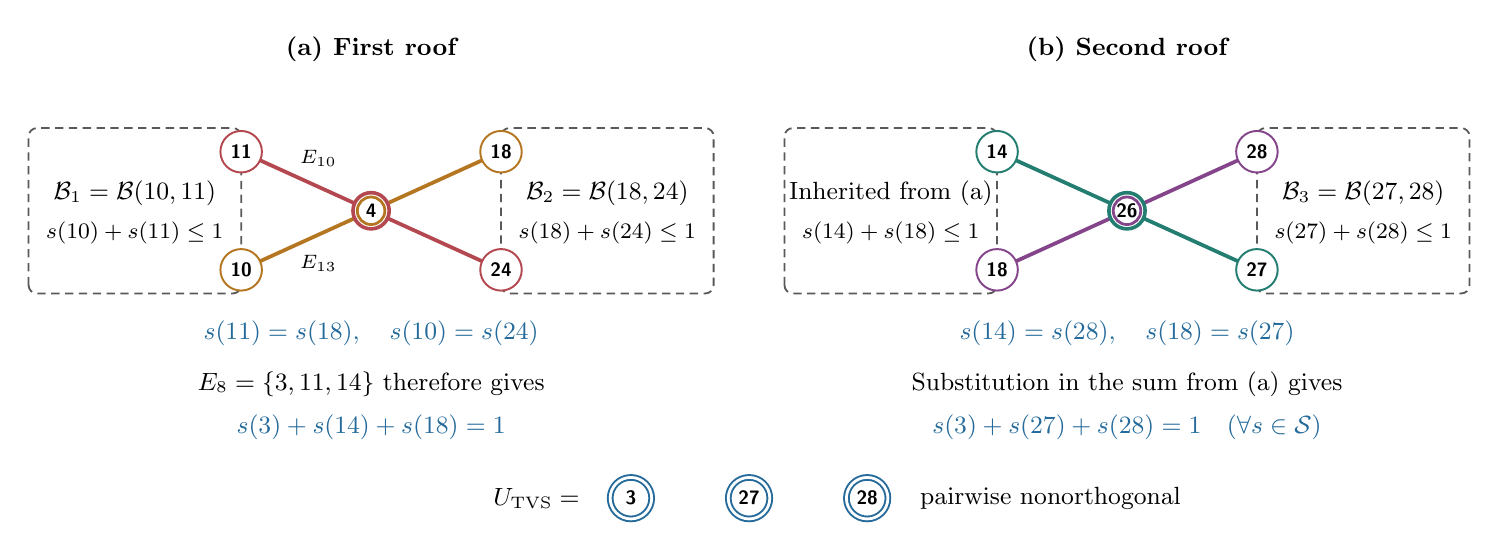
\begin{tikzpicture}[x=1cm,y=1cm,
  rooftrace/.style={line width=1.35pt,line cap=round},
  roofbox/.style={draw=black!65,densely dashed,line width=.65pt,rounded corners=3pt},
  roofnumber/.style={circle,draw=black,fill=white,line width=.7pt,
    minimum size=15pt,inner sep=0pt,font=\sffamily\bfseries\scriptsize},
  rooftext/.style={font=\small,align=center},
  roofresult/.style={font=\small,align=center,text=YOtriad},
  rooftitle/.style={font=\bfseries\small}]
  % The panels display the same two-context logic with different labels.
  % Box boundaries compress bugs or an inherited inequality; they are not contexts.
  \begin{scope}[shift={(-4.8,0)}]
    \node[rooftitle] at (0,2.05) {(a) First roof};
    \draw[roofbox] (-4.35,-1.05) rectangle (-1.65,1.05);
    \draw[roofbox] (1.65,-1.05) rectangle (4.35,1.05);
    \node[rooftext] at (-3,.22) {$\mathcal B_1=\mathcal B(10,11)$};
    \node[font=\footnotesize] at (-3,-.28) {$s(10)+s(11)\le1$};
    \node[rooftext] at (3,.22) {$\mathcal B_2=\mathcal B(18,24)$};
    \node[font=\footnotesize] at (3,-.28) {$s(18)+s(24)\le1$};
    % Each context bends at its shared roof vertex.
    \draw[rooftrace,YOctx10] (-1.65,.75)--(0,0)--(1.65,-.75);
    \draw[rooftrace,YOctx13] (-1.65,-.75)--(0,0)--(1.65,.75);
    \node[font=\scriptsize,fill=white,inner sep=1.2pt] at (-.67,.67) {$E_{10}$};
    \node[font=\scriptsize,fill=white,inner sep=1.2pt] at (-.67,-.67) {$E_{13}$};
    \node[roofnumber,draw=YOctx10] at (-1.65,.75) {11};
    \node[roofnumber,draw=YOctx13] at (-1.65,-.75) {10};
    \node[roofnumber,draw=YOctx13] at (1.65,.75) {18};
    \node[roofnumber,draw=YOctx10] at (1.65,-.75) {24};
    \draw[YOctx10,line width=1.3pt,fill=white] (0,0) circle[radius=.23];
    \draw[YOctx13,line width=1pt] (0,0) circle[radius=.175];
    \node[font=\sffamily\bfseries\scriptsize] at (0,0) {4};
    \node[roofresult] at (0,-1.55) {$s(11)=s(18),\quad s(10)=s(24)$};
    \node[rooftext] at (0,-2.20) {$E_8=\{3,11,14\}$ therefore gives};
    \node[roofresult] at (0,-2.75) {$s(3)+s(14)+s(18)=1$};
  \end{scope}
  \begin{scope}[shift={(4.8,0)}]
    \node[rooftitle] at (0,2.05) {(b) Second roof};
    \draw[roofbox] (-4.35,-1.05) rectangle (-1.65,1.05);
    \draw[roofbox] (1.65,-1.05) rectangle (4.35,1.05);
    \node[rooftext] at (-3,.22) {Inherited from (a)};
    \node[font=\footnotesize] at (-3,-.28) {$s(14)+s(18)\le1$};
    \node[rooftext] at (3,.22) {$\mathcal B_3=\mathcal B(27,28)$};
    \node[font=\footnotesize] at (3,-.28) {$s(27)+s(28)\le1$};
    \draw[rooftrace,YOctx5] (-1.65,.75)--(0,0)--(1.65,-.75);
    \draw[rooftrace,YOctx16] (-1.65,-.75)--(0,0)--(1.65,.75);
    \node[roofnumber,draw=YOctx5] at (-1.65,.75) {14};
    \node[roofnumber,draw=YOctx16] at (-1.65,-.75) {18};
    \node[roofnumber,draw=YOctx16] at (1.65,.75) {28};
    \node[roofnumber,draw=YOctx5] at (1.65,-.75) {27};
    \draw[YOctx5,line width=1.3pt,fill=white] (0,0) circle[radius=.23];
    \draw[YOctx16,line width=1pt] (0,0) circle[radius=.175];
    \node[font=\sffamily\bfseries\scriptsize] at (0,0) {26};
    \node[roofresult] at (0,-1.55) {$s(14)=s(28),\quad s(18)=s(27)$};
    \node[rooftext] at (0,-2.20) {Substitution in the sum from (a) gives};
    \node[roofresult] at (0,-2.75) {$s(3)+s(27)+s(28)=1\quad(\forall s\in\mathcal S)$};
  \end{scope}
  % Three separate markers, without connecting lines: the target is not a context.
  \node[font=\small] at (-2.7,-3.65) {$U_{\mathrm{TVS}}=$};
  \foreach \vx/\name in {-1.5/3,0/27,1.5/28}{
    \node[roofnumber,double,double distance=1pt,draw=YOtriad] at (\vx,-3.65) {\name};
  }
  \node[font=\small,anchor=west] at (2.05,-3.65) {pairwise nonorthogonal};
\end{tikzpicture}%
}
\caption{The two applications of the roof-twin lemma in Theorem~\ref{thm:tvs-admissibility}. Each solid trace contains one complete three-vertex roof context; their shared numbered circle is the roof vertex. Dashed boxes compress seven-context bugs, except the left box in (b), which records the inequality inherited from (a). Box boundaries are not contexts. The compressed bugs are $\mathcal B_1=\mathcal B(10,11;0)$, $\mathcal B_2=\mathcal B(18,24;100)$, and $\mathcal B_3=\mathcal B(27,28;200)$; their internal vertices are omitted. In (a), $\{4,11,24\}$ and $\{4,10,18\}$ force the first twins; context $\{3,11,14\}$ then gives the sum shown below. In (b), $\{26,14,27\}$ and $\{26,18,28\}$ force the second twins, yielding normalization on $U_{\mathrm{TVS}}$. The three separate double-outlined markers identify that target triple without adding a context or orthogonality relation. Repeated numbers in the panels refer to the same rays. This is a logical schematic common to $G_{41,25}$ and $G_{41,26}$; the extra context $\{4,5,105\}$ of the latter is omitted. The proof and coordinate certificate establish the full faithful geometry independently of this drawing.}\label{fig:TVS-admissibility}
\end{figure*}
% --- end verbatim ---

The spectra show the same two-sided pattern as before. On every two-valued state of either $41$-ray hypergraph the total on $U_{\mathrm{TVS}}$ is one, while $P_3+P_{27}+P_{28}$ has the quantum ranges
\begin{equation}\label{eq:classical-roof-intervals}
\begin{aligned}
G_{41,25}:&\quad[0.79852694,1.21074603],\\
G_{41,26}:&\quad[0.68238324,1.35933946]
\end{aligned}
\end{equation}
in the respective representations. The twin identities are violated as well.

% --- verbatim from long version ---
For $G_{41,26}$, the identity $s(11)=s(18)$ gives the particularly simple classical equality $p(11)=p(18)$ on every two-valued mixture. The quantum difference is
\begin{equation}\label{eq:G41-exact-twin-operator}
P_{11}-P_{18}=\frac16\begin{pmatrix}1&-1&0\\-1&1&0\\0&0&-2\end{pmatrix},
\end{equation}
whose eigenvalues are $-1/3,0,1/3$. The preparation $\psi=(1,-1,0)^{\mathsf T}/\sqrt2$ attains
\begin{equation}\label{eq:G41-exact-twin-witness}
p_\psi(11)=\frac23,\qquad p_\psi(18)=\frac13,
\end{equation}
so the maximal absolute violation of this equality is exactly $1/3$.
% --- end verbatim ---

% ==================================================================
\section{Completeness on color classes only}\label{sec:complete-rainbow}
% ==================================================================
We now turn to the weakest level. A chromatic admissible context is normalized on the extendable states; nothing is required of the other two-valued states. The following theorem expresses this, and two related relations, through colors. Two vertices are \emph{chromatic twins}, written $u\sim_c v$, if $c(u)=c(v)$ for every $c\in\Cc_d(H)$. Two disjoint sets $A,B\subseteq V$ of equal size are \emph{color-multiset equivalent} if they carry the same multiset of colors in every strong $d$-coloring.

% --- verbatim from long version ---
\begin{theorem}[Chromatic Relations via Extendable State Sums]\label{thm:chromatic-conservation}
Let $H=(V,E)$ be a $d$-uniform hypergraph with $\Cc_d(H)\neq\varnothing$ and extendable state set $\Sc_{\mathrm{ext}}(H)=\{s_j=\mathbf{1}_{c^{-1}(\{j\})}:c\in\Cc_d(H),\,0\le j\le d-1\}$. Then:
\begin{enumerate}
\item A $d$-element set $U=\{u_1,\ldots,u_d\}\subseteq V$ satisfies $\{c(u):u\in U\}=\{0,\ldots,d-1\}$ for all $c\in\Cc_d(H)$ if and only if
\begin{equation}\label{eq:thm-complete-state}
\sum_{u\in U} s(u) = 1 \qquad \forall\, s\in\Sc_{\mathrm{ext}}(H).
\end{equation}
\item A $k$-element set $U=\{u_1,\ldots,u_k\}\subseteq V$ ($2\le k<d$) satisfies $c(u_a)\neq c(u_b)$ ($a\neq b$) for all $c\in\Cc_d(H)$ if and only if
\begin{equation}\label{eq:thm-subcomplete-state}
\sum_{u\in U} s(u) \le 1 \qquad \forall\, s\in\Sc_{\mathrm{ext}}(H).
\end{equation}
\item Disjoint $k$-element sets $A,B\subseteq V$ satisfy $\{\!\{c(a):a\in A\}\!\}=\{\!\{c(b):b\in B\}\!\}$ for all $c\in\Cc_d(H)$ if and only if
\begin{equation}\label{eq:thm-paired-state}
\sum_{a\in A} s(a) = \sum_{b\in B} s(b) \qquad \forall\, s\in\Sc_{\mathrm{ext}}(H).
\end{equation}
\end{enumerate}
\end{theorem}
\begin{proof}
For any $c\in\Cc_d(H)$, let $s_j=\mathbf{1}_{c^{-1}(\{j\})}\in\Sc_{\mathrm{ext}}(H)$ ($0\le j\le d-1$) be the indicator functions of its $d$ color classes. For any subset $X\subseteq V$ and color $j\in\{0,\ldots,d-1\}$, the sum
\begin{equation}\label{eq:multiplicity-identity}
\sum_{x\in X} s_j(x) = \bigl|\{x\in X: c(x)=j\}\bigr|
\end{equation}
counts the exact multiplicity of color $j$ on $X$ in coloring $c$.
(1) When $|U|=d$, every color $j\in\{0,\ldots,d-1\}$ has multiplicity $1$ on $U$ iff $\{c(u):u\in U\}=\{0,\ldots,d-1\}$, establishing Eq.~\eqref{eq:thm-complete-state}.
(2) Every color $j$ has multiplicity at most $1$ on $U$ iff no two elements of $U$ share a color in $c$, establishing Eq.~\eqref{eq:thm-subcomplete-state}.
(3) By Eq.~\eqref{eq:multiplicity-identity}, color $j$ has the same multiplicity on $A$ and on $B$ for every $j\in\{0,\ldots,d-1\}$ and every $c\in\Cc_d(H)$ iff $\sum_{a\in A}s_j(a)=\sum_{b\in B}s_j(b)$ for every $s_j\in\Sc_{\mathrm{ext}}(H)$, establishing Eq.~\eqref{eq:thm-paired-state}.
\end{proof}
% --- end verbatim ---

\subsection{A Yu--Oh restriction}\label{sec:H21-rainbow}
Let $H_{21,13}$ consist of the four base contexts
\begin{equation}\label{eq:H21-base}
\{1,2,3\},\quad\{4,5,6\},\quad\{7,8,9\},\quad\{2,5,8\}
\end{equation}
of the completed Yu--Oh configuration~\cite{Yu-2012,svozil-2026-chromaticcoordinatization} together with three of its four diagonal sectors, with hubs $10$, $11$, and $13$:
\begin{equation}\label{eq:H21-sectors}
\begin{gathered}
\{9,10,23\},\quad\{1,10,19\},\quad\{4,10,18\},\\
\{3,11,14\},\quad\{7,11,15\},\quad\{4,11,24\},\\
\{1,13,20\},\quad\{7,13,21\},\quad\{6,13,22\}.
\end{gathered}
\end{equation}
The first two sectors and the three contexts $\{1,2,3\}$, $\{7,8,9\}$, $\{2,5,8\}$ form the hypergraph $I_{16,9}$ of Eq.~\eqref{eq:I16-def}. A faithful representation of $H_{21,13}$ in $\R^3$ is given by
\begin{equation}\label{eq:YO-rays}
\begin{aligned}
r_1&=(0,1,1),&r_2&=(1,0,0),\\
r_3&=(0,1,-1),&r_4&=(1,1,0),\\
r_5&=(0,0,1),&r_6&=(1,-1,0),\\
r_7&=(1,0,1),&r_8&=(0,1,0),\\
r_9&=(1,0,-1),&r_{10}&=(1,-1,1),\\
r_{11}&=(1,-1,-1),&r_{13}&=(1,1,-1),
\end{aligned}
\end{equation}
and, for the third ray of each sector context, the cross product of the other two; for instance $r_{24}=r_4\times r_{11}\propto(1,-1,2)$. Of the $\binom{21}{2}=210$ pairs of rays, exactly the $39$ pairs sharing a context are orthogonal. The fourth Yu--Oh hub $r_{12}=(1,1,1)$ is omitted. There are $21$ two-valued states, six of them extendable.

% --- verbatim from long version ---
\begin{lemma}[Structural Color Propagation in $H_{21,13}$]\label{lem:H21-structural}
Every strong $3$-coloring gives distinct colors to the hubs $10,11,13$ and to each of the triples $\{1,4,7\}$ and $\{3,6,9\}$. There are exactly two normalized strong $3$-colorings, representing all $12$ labeled colorings.
\end{lemma}
\begin{proof}
Suppose first that hubs $10,11$ share color $t$. Vertices $1,3$ both avoid $t$, so their context forces $c(2)=t$. Similarly, vertices $7,9$ both avoid $t$, forcing $c(8)=t$, contrary to the context $\{2,5,8\}$. Equating hubs $10,13$ similarly forces $c(5)=c(8)$, while equating $11,13$ forces $c(2)=c(5)$. Thus the hub triple is rainbow.

Adjacency to two hubs now forces
\[
c(1)=c(11),\quad c(4)=c(13),\quad c(7)=c(10),
\]
so $\{1,4,7\}$ is rainbow. Arrange the three base contexts as rows of
\[
\begin{pmatrix}1&2&3\\4&5&6\\7&8&9\end{pmatrix}.
\]
Every row contains each color once. The first column is rainbow by the preceding argument, and the middle column is an actual context. Counting occurrences of each color therefore leaves exactly one occurrence in the last column, proving that $\{3,6,9\}$ is rainbow.

Normalize the middle column to $(0,1,2)$. The first column is a permutation avoiding the middle-column color in each row, so it is one of the two derangements of three colors. The last column, the hubs, and every remaining vertex are then uniquely determined. Both derangements extend to all contexts. Hence there are two normalized colorings, and their six color permutations exhaust all $12$ labeled strong colorings.
\end{proof}
% --- end verbatim ---

\begin{proposition}[Chromatic Admissible Triples in $H_{21,13}$]\label{prop:H21-triples}
The pairwise nonorthogonal triples
\begin{equation}\label{eq:H21-triples}
\begin{gathered}
U_{\mathrm{hub}}=\{10,11,13\},\qquad U_{\mathrm{core}}=\{1,4,7\},\\
U_{\mathrm{cop}}=\{3,6,9\}
\end{gathered}
\end{equation}
are chromatic admissible contexts of $H_{21,13}$. None of them is normalized on all two-valued states: the restrictions of the $21$ states to $U_{\mathrm{hub}}$ are $000,100,010,001$, and those to $U_{\mathrm{core}}$ and to $U_{\mathrm{cop}}$ are all binary triples except $111$. Altogether $H_{21,13}$ has $21$ chromatic admissible contexts.
\end{proposition}
\begin{proof}
By Lemma~\ref{lem:H21-structural} the three triples are rainbow in every strong coloring, and Theorem~\ref{thm:chromatic-conservation}(1) converts this into normalization on $\Sc_{\mathrm{ext}}(H_{21,13})$. Pairwise nonorthogonality is read off Eq.~\eqref{eq:YO-rays}. The state restrictions and the total count follow from enumerating the $21$ two-valued states and the two normalized colorings.
\end{proof}
The three triples compare differently with quantum probabilities. The hubs are pairwise exclusive on \emph{all} two-valued states, so $p(10)+p(11)+p(13)\le1$ holds for every classical mixture. The spectrum of $P_{10}+P_{11}+P_{13}$ is $\{1/3,4/3,4/3\}$, and the preparation
\begin{equation}\label{eq:H21-hub-explicit-witness}
\begin{aligned}
\psi_{\mathrm{hub}}&=(1,-1,0)^{\mathsf T}/\sqrt2,\\
\bigl(p(10),p(11),p(13)\bigr)&=(2/3,2/3,0)
\end{aligned}
\end{equation}
violates that inequality with total $4/3$. For $U_{\mathrm{core}}$ and $U_{\mathrm{cop}}$ the spectra are $\{1/2,1/2,2\}$ and $\{0,3/2,3/2\}$; the rays of $U_{\mathrm{cop}}$ are coplanar, $r_3+r_6-r_9=0$. Their quantum totals depart from the color-class value one, as Proposition~\ref{prop:two-sided} requires, but stay within the range $[0,2]$ allowed by all two-valued states. These two triples therefore separate quantum predictions from common-spectrum labelings only.

Deleting the roof context $\{6,13,22\}$ gives a $20$-ray, $12$-context hypergraph $H_{20,12}$ with $N_c=4$ and two chromatic admissible contexts, $\{15,18,20\}$ and $\{19,21,24\}$. On its $25$ two-valued states their totals range from one to three, so every classical mixture has total at least one. Because $r_6\perp r_{13}$ in Eq.~\eqref{eq:YO-rays}, this hypergraph needs its own faithful representation, for instance
\begin{equation}\label{eq:H20-rays}
\begin{aligned}
r_1&=(0,1,2),&r_2&=(1,0,0),\\
r_3&=(0,2,-1),&r_4&=(1,1,0),\\
r_5&=(0,0,1),&r_6&=(1,-1,0),\\
r_7&=(2,0,1),&r_8&=(0,1,0),\\
r_9&=(1,0,-2),&r_{10}&=(2,-2,1),\\
r_{11}&=(1,-1,-2),&r_{13}&=(1,4,-2),\\
r_{14}&=(5,1,2),&r_{15}&=(1,5,-2),\\
r_{18}&=(1,-1,-4),&r_{19}&=(5,4,-2),\\
r_{20}&=(-10,2,-1),&r_{21}&=(-4,5,8),\\
r_{23}&=(4,5,2),&r_{24}&=(1,-1,1).
\end{aligned}
\end{equation}
In this representation both triples have the spectrum $\{0.72960967,1.03555226,1.23483806\}$, so the quantum total can fall below the classical lower bound one. An exhaustive search over all nonempty context subsets of $H_{21,13}$ finds no pairwise nonorthogonal triple that is rainbow in every strong coloring with fewer than $12$ contexts. The three $12$-context subsets that have one arise by deleting $\{6,13,22\}$, $\{3,11,14\}$, or $\{9,10,23\}$, and each carries the same two triples.

% ==================================================================
\section{Affine pseudocontexts force equal color multisets}\label{sec:paired-affine}
% ==================================================================
At the strongest level an identity follows linearly from the context equations and therefore holds for all Born probabilities. By Proposition~\ref{prop:no-operator-complete} this cannot happen for a single independent $d$-set. It does happen for pairs of sets, the affine pseudocontexts of Ref.~\cite{2026-Navara-Svozil-pseudocontexts}, and these leave a trace at the color level.

% --- verbatim from long version ---
\begin{corollary}[Affine Pseudocontexts Imply Color-Multiset Equivalence]\label{cor:affine-to-chromatic}
Let $M_H\in\{0,1\}^{n\times |V|}$ be the context-vertex incidence matrix of $H$. If disjoint nonorthogonal $k$-tuples $A,B\subseteq V$ admit a balanced context certificate $\lambda\in\R^n$ satisfying~\cite{2026-Navara-Svozil-pseudocontexts}
\begin{equation}\label{eq:balanced-certificate}
M_H^{\mathsf T}\lambda = \chi_A - \chi_B,\qquad \mathbf{1}_n^{\mathsf T}\lambda = 0,
\end{equation}
then in every strong $d$-coloring $c\in\Cc_d(H)$, $A$ and $B$ carry the exact same multiset of colors: $\{\!\{c(a):a\in A\}\!\}=\{\!\{c(b):b\in B\}\!\}$.
\end{corollary}
\begin{proof}
Every extendable state $s\in\Sc_{\mathrm{ext}}(H)\subseteq\Sc(H)$ satisfies $M_H s=\mathbf{1}_n$, so
\[
\sum_{a\in A}s(a)-\sum_{b\in B}s(b)=(\chi_A-\chi_B)^{\mathsf T}s=\lambda^{\mathsf T}M_H s=\lambda^{\mathsf T}\mathbf{1}_n=0.
\]
Applying Theorem~\ref{thm:chromatic-conservation}(3) completes the proof.
\end{proof}
% --- end verbatim ---

\subsection{Examples}\label{sec:B13-R21}
Known examples are Mayet's $15$-ray configuration in $\R^3$, with paired triples, and a $20$-ray octagon in $\C^3$, with paired sets of size two~\cite{Navara_1995,Mayet_2000,2023-navara-svozil,2026-Navara-Svozil-pseudocontexts}. Two further ones use configurations already at hand.

\emph{Specker bug.} In the bug $\mathcal B(10,11;0)$ of Eq.~\eqref{eq:roof-bug-contexts}, with the coordinates of Eq.~\eqref{eq:YO-rays}, write $E_1=\{1,2,3\}$, $E_2=\{7,8,9\}$, $E_4=\{3,11,14\}$, $E_5=\{7,11,15\}$, $E_6=\{9,10,23\}$, and $E_7=\{1,10,19\}$. Then
\begin{equation}\label{eq:B13-paired3}
\begin{aligned}
\chi_A-\chi_B&=(\chi_{E_1}+\chi_{E_5}+\chi_{E_6})\\
&\quad-(\chi_{E_2}+\chi_{E_4}+\chi_{E_7}),\\
A&=\{2,15,23\},\qquad B=\{8,14,19\}.
\end{aligned}
\end{equation}
Hence $p(2)+p(15)+p(23)=p(8)+p(14)+p(19)$ for all Born probabilities, and both triples carry the same color multiset in each of the $N_c=6$ strong colorings.

\emph{Row--column hub grids.} Arrange nine vertices in three rows $R_1=\{1,2,3\}$, $R_2=\{4,5,6\}$, $R_3=\{7,8,9\}$, and attach each grid column to one of the hubs $10$, $11$, $12$ through the hub contexts
\begin{equation}\label{eq:R21-hub-contexts}
\begin{gathered}
\{1,10,13\},\quad\{2,11,14\},\quad\{3,12,15\},\\
\{4,10,16\},\quad\{5,11,17\},\quad\{6,12,18\},\\
\{7,10,19\},\quad\{8,11,20\},\quad\{9,12,21\}.
\end{gathered}
\end{equation}
The three rows and nine hub contexts form $R_{21,12}$, with $N_c=32$ and $|\Sc_{\mathrm{ext}}|/|\Sc|=48/54$. Adding an apex $22$ through
\begin{equation}\label{eq:R25-extra-contexts}
\{22,10,23\},\quad\{22,11,24\},\quad\{22,12,25\}
\end{equation}
gives $R_{25,15}$, with $N_c=24$ and $|\Sc_{\mathrm{ext}}|/|\Sc|=48/81$. The labels of this example are independent of those used above. A faithful representation in $\C^3$ with Gaussian-integer coordinates is

% --- verbatim from long version ---
\begin{equation}\label{eq:R25-gaussian-vectors}
\begin{aligned}
r_1&=(1,0,0),&r_2&=(0,1,0),\\
r_3&=(0,0,1),&r_4&=(-1+i,2,2),\\
r_5&=(2,-1+i,2),&r_6&=(2,2,-1+i),\\
r_7&=(-1-2i,2,2),&r_8&=(2,-1-2i,2),\\
r_9&=(2,2,-1-2i),&r_{10}&=(0,1,-1),\\
r_{11}&=(-1,0,1),&r_{12}&=(1,-1,0),\\
r_{13}&=(0,1,1),&r_{14}&=(1,0,1),\\
r_{15}&=(1,1,0),&r_{16}&=(2-2i,1,1),\\
r_{17}&=(1,2-2i,1),&r_{18}&=(1,1,2-2i),\\
r_{19}&=(4,1-2i,1-2i),&r_{20}&=(1-2i,4,1-2i),\\
r_{21}&=(1-2i,1-2i,4),&r_{22}&=(1,1,1),\\
r_{23}&=(2,-1,-1),&r_{24}&=(-1,2,-1),\\
r_{25}&=(-1,-1,2).&&
\end{aligned}
\end{equation}
% --- end verbatim ---

All $25$ rays are distinct, and two of them are orthogonal exactly when they share one of the listed contexts; the first $21$ rays represent $R_{21,12}$.


% --- verbatim from long version ---
Write $H_{ij}$ for the listed hub context incident with the $j$th core vertex of row $R_i$.

Choosing two distinct rows and one column gives $\binom32\cdot3=9$ unordered size-three affine pseudocontext pairs. For rows $R_1,R_2$ and column $1$, the two $3$-context families are
\begin{equation}\label{eq:R21-three-coverings}
\begin{aligned}
\mathcal F_+&=\{R_1,H_{22},H_{23}\},\\
\mathcal F_-&=\{R_2,H_{12},H_{13}\}.
\end{aligned}
\end{equation}
Their incidence difference is $\sum_{C\in\mathcal F_+}\chi_C-\sum_{C\in\mathcal F_-}\chi_C=\chi_A-\chi_B$, where
\begin{equation}\label{eq:R21-paired3}
A=\{1,17,18\},\qquad B=\{4,14,15\}.
\end{equation}
The other three pairs compare the tip triples $T_1=\{13,14,15\}$, $T_2=\{16,17,18\}$, and $T_3=\{19,20,21\}$. They have balanced $4$-context certificates
\begin{equation}\label{eq:R21-four-coverings}
\begin{aligned}
\chi_{T_i}-\chi_{T_k}
&=\chi_{R_k}+\sum_{j=1}^3\chi_{H_{ij}}\\
&\quad-\chi_{R_i}-\sum_{j=1}^3\chi_{H_{kj}},\qquad i<k.
\end{aligned}
\end{equation}
Together these give all $12$ size-three affine pairs in each graph.
% --- end verbatim ---

Their certificates force equal color multisets on both sides in every strong coloring. In $R_{21,12}$ the six nonextendable states are exactly those that select one grid vertex in each row and each column.

% ==================================================================
\section{Summary}\label{sec:conclusion}
% ==================================================================
Two-valued states can force pairwise nonorthogonal rays to be exclusive and complete. In $H_{53,34}$ and in the two $41$-ray configurations this holds for every two-valued state, although the projectors do not sum to the identity. Every noncontextual value assignment thus treats the triple as a context, while the quantum total ranges over an interval around one: approximately $[0.571,1.517]$ in $H_{53,34}$. By Proposition~\ref{prop:two-sided} such a two-sided violation is unavoidable.

The examples separate three levels. On color classes only: the core and coplanar triples of $H_{21,13}$, whose quantum totals contradict common-spectrum labelings but no general noncontextual model. On all two-valued states: the triples of $H_{53,34}$, $G_{41,25}$, and $G_{41,26}$; the hub exclusivity in $H_{21,13}$, violated with total $4/3$; and twin identities such as $p(11)=p(18)$ in $G_{41,26}$, violated by $1/3$. On the affine level: no single set, but pairs of sets, whose identities hold for all Born probabilities and force equal color multisets.

The mechanism is the binary range of two-valued states, acting through Specker bugs. It makes the affine hull of the two-valued states strictly smaller than the solution space of the context equations, and quantum probabilities use the difference. All witnesses are state dependent, and their numerical values depend on the chosen faithful representation. No minimality is claimed for $53$ or $41$ rays.

% --- verbatim from long version ---
\begin{acknowledgments}
This research was funded in part by the Austrian Science Fund (FWF), Grant DOI \href{https://doi.org/10.55776/PIN5424624}{10.55776/PIN5424624}.
\end{acknowledgments}

\def\doibase{https://doi.org/}
\bibliography{svozil}

\end{document}
% --- end verbatim ---
